\documentclass[11pt,a4paper]{article}

% Packages
\usepackage{fontspec}
\setmainfont{Hiragino Mincho ProN}
\setsansfont{Hiragino Kaku Gothic ProN}
\setmonofont{Menlo}
\usepackage{iftex}
\ifXeTeX
  \XeTeXlinebreaklocale "ja"
  \XeTeXlinebreakskip=0pt plus 1pt minus 0.1pt
\fi
\usepackage{amsmath,amssymb,amsthm}
\usepackage{graphicx}
\usepackage{hyperref}
\usepackage{booktabs}

\newtheorem{theorem}{定理}
\newtheorem{definition}{定義}

\title{情報損失としての構造崩壊：\\累積制約下の指数減衰メカニズム}
\author{Akihito Sunagawa\thanks{akihito.sunagawa@gmail.com}}
\date{2026年3月}

\begin{document}

\maketitle

\begin{abstract}
大規模言語モデル（LLM）は、構造的矛盾がコンテキストに蓄積すると推論が突然崩壊する---事実的ノイズ下での緩やかな劣化とは質的に異なる現象である。制御された実験（5ベンダーの11モデル、4B--70B以上のパラメータ）を通じてこの崩壊を特徴づけ、以下を発見した：(i) コンテキストマージン（$\mu$）と構造的矛盾（$\delta$）の間の乗法的交互作用---個別には致死的でない2つのストレッサーが組み合わさると致死的になり、加法的劣化モデルを排除する；(ii) $\delta$における次元構造---十分なベースライン精度を持つモデルにおいて、単一の構造的矛盾が10個の事実的矛盾よりも大きな損害を与える；(iii) クッション機構---RLHFアラインメントが矛盾を圧倒されるまで吸収し、システム固有の臨界閾値$\delta_c$を生じる。

これらのパターンは組合せ論の第一モーメント法により説明される。累積情報損失$\delta = \sum_i I(\text{constraint}_i)$をナット単位で定義すると、乗法的存続ポテンシャル
\[
S = N_{eff} \cdot \frac{\mu}{\mu_c} \cdot e^{-\delta}
\]
はLLMの崩壊パターンを捉えるとともに、$\delta$が正確に計算可能なブール充足可能性（SAT）においてパラメータフリー予測を与える：減衰率比$\alpha_{\text{XOR}}/\alpha_{\text{random}} = \ln 2 / |\ln(7/8)| = 5.19\times$は上界であり、実験的に確認された（観測値：$5.04 \pm 0.25$、CV $= 5\%$；系統的な下方偏差は制約間相関が有効情報損失を減少させることと整合する---制約の重複が冗長性を生み、一箇所の違反がシステム全体に与える影響を緩和する）。指数ペナルティ$e^{-\delta}$は近似ではなく、SAT解の個数の第一モーメントとの数学的恒等式である。その貢献は操作的方法論---構造的矛盾を第一モーメント対応を通じてナット単位の情報損失として測定すること---であり、2つの制御されたドメインで検証された。

\medskip
\noindent\textbf{キーワード：} LLM推論崩壊、構造的矛盾、情報損失、乗法モデル、SAT相転移、生存分析、形式検証
\end{abstract}

%=============================================
\section{はじめに}

情報を処理するシステムは、内部矛盾が蓄積すると突然失敗しうる。大規模言語モデルにおいて、これは突然の推論崩壊として現れる：十分なベースライン精度を持つモデルにおいて、単一の構造的矛盾---自己言及パラドックス、メタレベルの不整合---が10個の事実的矛盾よりも大きな損害を与える（第\ref{sec:llm-delta-structure}節）。個別には無害な2つのストレッサー（適度なコンテキスト負荷と適度な矛盾）が組み合わさると致死的になる（第\ref{sec:llm}節）。4Bから70B以上のパラメータを持つ5ベンダーの11モデルにわたり再現された（第\ref{sec:cross-model}節）これらのパターンは、注意機構の劣化や誤差伝播のような加法的劣化モデルでは説明できない---それらは各ストレッサーに独立に比例するパフォーマンス低下を予測する。この現象は、再帰的訓練データ下でのモデル崩壊\cite{shumailov2024}（分布の狭窄として現れる累積情報損失）とは関連しつつも区別される。

なぜ加法的ではなく乗法的なのか？ 本稿はその答えが組合せ論の第一モーメント法という既知の数学的構造にあると提案する。\textbf{累積情報損失}$\delta = \sum_i I(\text{constraint}_i)$をナット単位で定義し、各構造的制約が計算可能な量の情報損失を寄与する。存続ポテンシャルは次の通りである：
\begin{equation}
S = N_{eff} \cdot \frac{\mu}{\mu_c} \cdot e^{-\delta}
\label{eq:survival}
\end{equation}
ここで$N_{eff}$は有効選択肢数（システムが利用可能な独立した代替選択肢の数）、$\mu/\mu_c$は臨界閾値に対するマージン、$e^{-\delta}$は蓄積された構造的矛盾からの指数ペナルティである。いずれかの因子がゼロに近づけば他に関係なく致命的になるこの乗法構造は、直列信頼性\cite{barlow1975}、原子炉臨界\cite{duderstadt1976}、および感染症閾値（$R_0$）の構造である。注目すべきことに、同様の分離は信用評価において独立に制度化されている：主要格付機関（S\&P、Moody's、Fitch）は定量的財務健全性（$\mu$）と定性的ガバナンス要因（$\delta$）を区別しており、Moody'sは「支払能力」と「支払意思」を明示的に分離する---理論的動機なしに数十年の実務を通じて到達したキャパシティ--制約分解である\cite{cantor1996}。

本稿の貢献は乗法構造そのものではなく、情報理論的基盤付けにある：$\delta$を第一モーメント法を通じてナット単位で操作的に定義することで、制約の量だけでなく質が第一原理から計算可能になる。ブール充足可能性（SAT）において、$e^{-\delta}$は解の個数の第一モーメントと数学的に同一である（第\ref{sec:first-moment}節）。この恒等式はパラメータフリー予測を与える：XOR制約はランダム節の$\ln 2 / \ln(8/7) \approx 5.19$倍低い密度で崩壊を引き起こすはずであり---$5.04 \pm 0.25$で実験的に確認された（CV $= 5\%$；第\ref{sec:sat}節）。同じ数学的構造が、LLMにおいて構造的矛盾が事実的ノイズよりも質的に大きな損害を与える理由を説明する：制約あたりの情報損失がより大きいのである。

\subsection{研究課題}

\begin{enumerate}
    \item \textbf{操作的定義}：構造的矛盾を、確立された数学との正確な対応を持つ情報損失（$\delta$、ナット単位）として測定できるか？
    \item \textbf{乗法構造}：$N_{eff}$、$\mu/\mu_c$、$e^{-\delta}$は（直列信頼性のように）乗法的に結合するか、それとも加法的か？
    \item \textbf{予測}：この枠組みはパラメータフリーで反証可能な予測を生成し、制御された実験で成立するか？
\end{enumerate}

\subsection{2つの精度レベル}

適用可能性の2つのレベルを区別する：

\begin{itemize}
    \item \textbf{レベルA}（外部定義された存続）：存続がシステム自体から独立に定義され、$\delta$が直接計算可能なシステム。SATインスタンス（充足可能性）およびLLM実験（正解の生成）がこのレベルで動作する。予測は定量的に鋭い。

    \item \textbf{レベルB}（自己定義的存続）：存続条件がシステム自身のアイデンティティに依存し、$\delta$がプロキシ測定を必要とするシステム。企業、生物、生態系がこのレベルで動作する。予測は近似的であり、測定誤差$\varepsilon$に応じて$|S(\delta_{\text{meas}}) - S(\delta_{\text{true}})| \leq N_{eff} \cdot \varepsilon \cdot (\mu/\mu_c)$で形式的に上界される。
\end{itemize}

本稿はレベルAの証拠（SAT実験およびLLM実験）に焦点を当てる。これらでは$\delta$が正確にまたはほぼ正確に計算可能である。

\subsection{なぜ2つのドメインが必要か}

どちらのドメインも単独では不十分である。SATは$e^{-\delta}$成分---累積情報損失と解数の第一モーメントの間の数学的恒等式---を検証するが、$\mu$と$\delta$の乗法的相互作用をテストできない。SATにはマージンという変数が存在しないためである。LLM実験は乗法的$\mu \times \delta$相互作用を確認し、制約の質が量を支配することを明らかにするが、指数形式を独立に検証することはできない（低$\delta$領域では$e^{-\delta}$と$(1-\delta)^k$を識別できない）。したがって2つのドメインは相補的である：SATが数学を支え、LLMが乗法構造を支える。重要なことに、認識論的地位は異なる：SATでは、$e^{-\delta}$は第一モーメントとの\emph{数学的恒等式}（第\ref{sec:first-moment}節）である；LLMでは、同じ関数形式は\emph{構造的類推}であり、第一原理から導出されるのではなく経験的にテストされる。この区別は第\ref{sec:discussion}節で展開される。

\subsection{論文の構成}

第\ref{sec:related}節では先行する枠組みに対する本研究の位置づけを示す。第\ref{sec:theory}節では理論的枠組み：存続方程式、第一モーメント対応、指数ペナルティの導出を展開する。第\ref{sec:sat}節では3つの制約タイプとパラメータフリー予測に関するSAT実験を提示する。第\ref{sec:llm}節では乗法構造とクッション機構を確認する制御されたLLM実験を報告する。第\ref{sec:discussion}節では適用範囲、指数形式の限界、今後の方向性を議論する。第\ref{sec:limitations}節では具体的な限界を詳述する。第\ref{sec:conclusion}節で結論を述べる。

%=============================================
\section{関連研究}
\label{sec:related}

\subsection{生存分析とハザードモデル}

Cox比例ハザードモデル\cite{cox1972}は、Kaplan--Meier推定量\cite{kaplan1958}に基づき、生存分析の標準的枠組みを確立した：$h(t) = h_0(t) \exp(\beta' X)$。我々のモデルは指数形式を共有するが、重要な点で異なる：Coxモデルは共変量を回帰によって発見される事後的相関として扱うが、我々の枠組みは組合せ論における第一モーメント法から指数ペナルティ$e^{-\delta}$を導出し、指数部の構造的解釈を提供する。

\subsection{閾値現象と早期警告信号}

Schefferら\cite{scheffer2009}は、多くの複雑系が早期警告信号（増加する自己相関、分散、フリッカリング）に先行される臨界転移を示すことを確立した。May \cite{may1972}は生態系の安定性が多様性と接続性の関係に依存することを示した。我々の枠組みは、そのような転移の根底にある一つのメカニズムを形式化する：構造的矛盾の乗法的蓄積がシステムを臨界閾値に向かって駆動し、指数関数$e^{-\delta}$が蓄積された矛盾への非線形感度を捉える。

\subsection{散逸構造}

Prigogine \cite{prigogine1984}は、平衡から遠く離れた開放系が連続的なエネルギーと情報の流れを通じて構造を維持することを確立した。我々の存続方程式はそのような散逸構造に適用される：3つの因子（$N_{eff}$、$\mu/\mu_c$、$e^{-\delta}$）は散逸構造がエントロピー的崩壊に対して自己を維持する条件を分解する。

\subsection{情報理論的アプローチ}

Shannonの通信路符号化定理\cite{shannon1948,cover2006}は、信頼性のある通信にはチャネルの雑音率を超える冗長性が必要であることを確立した。組合せ論における第一モーメント法\cite{alon2016}は$\mathbb{E}[X] = 0 \implies \Pr[X > 0] = 0$を用いて非存在を証明する。我々の操作的定義$\delta = \sum_i I(\text{constraint}_i)$はこれらを接続する：各制約は情報（解、選択肢、容量）を除去し、$e^{-\delta}$は残存する期待される割合---すなわち第一モーメント上界そのものである。分子生物学において、Eigenのエラーカタストロフ\cite{eigen1971}は自己複製系の情報論的閾値を確立した：変異率が臨界値を超えると配列情報が不可逆的に失われる。閾値条件はナット単位で定式化されており、我々の$\delta_c$と構造的に同型である。主要な違いは、Eigenの$\delta$が単一ドメイン（RNA複製）における確率的コピーエラーから生じるのに対し、我々の枠組みは決定論的な構造的矛盾を扱い、構造的に異なる2つのドメインで検証されている点である。

独立に、Giannakopoulos \cite{giannakopoulos2025}は異なる出発点から指数的存続方程式$S(\eta) = \exp[-\alpha \cdot (1-\eta) \cdot Q/T]$を提案した（プレプリント、未査読）。

\subsection{LLMの推論崩壊}

Zhangら\cite{zhang2026lpt}は独立に、LLMの論理推論が急激な相転移を示すことを発見した---性能が特定の複雑性範囲内では安定し、その後急激に崩壊する現象で、「論理的相転移」（LPT）と名付けた。彼らの論理的複雑性メトリック（LoCM）は、重み付き演算子数、ネスト深度、推論ホップ数によりタスク難易度を定量化し、12以上のモデルで相転移パターンが観測された。

我々の研究は主に基盤付けの点で異なる：我々の$\delta = \sum_i I(\text{constraint}_i)$は第一モーメント対応を通じてナット単位で測定されるのに対し、LoCMは情報損失への接続を持たない経験的に較正された重みを使用する。このナットベースの枠組みにより、SAT、LLM、さらに原理的には組織や生態系にわたるクロスドメイン適用が単一の指標のもとで可能になる。

独立に、Apple ML Research \cite{apple2025illusion}は、標準LLMおよび推論強化LLMの両方が制御されたパズル環境において複雑性閾値を超えると急激な正解率崩壊を示すことを実証し、3つのレジーム（標準LLM優位、推論モデル優位、普遍的崩壊）を同定した。彼らの研究は崩壊閾値現象の独立した確認を提供するが、そのメカニズムに対する情報理論的枠組みは提示していない。

%=============================================
\section{理論的枠組み}
\label{sec:theory}

\subsection{存続方程式}

\begin{definition}[存続主体]
存続主体とは、蓄積する制約の下で内部整合性を維持する必要があり、崩壊（$S \to 0$）しうるシステムである。本稿では：SATインスタンス（崩壊 $=$ 充足不能）およびLLM推論セッション（崩壊 $=$ 正解を生成できない状態）。この形式主義は原理的には他の制約処理システム（生物、組織、生態系）にも拡張されるが、そのような拡張にはドメイン固有の$\delta$キャリブレーションが必要であり、本稿では検証されていない。
\end{definition}

存続ポテンシャル$S$は：
\begin{equation}
S = N_{eff} \cdot \frac{\mu}{\mu_c} \cdot e^{-\delta}
\label{eq:survival-main}
\end{equation}

\textbf{$S$はポテンシャルであり、確率ではない。}存続ポテンシャル$S$は$N_{eff} \cdot (\mu/\mu_c) > 1$のとき1を超えうる非正規化量である。存続条件は$S > S_c$（ドメイン固有の臨界閾値）であり、$S \in [0,1]$ではない。特定のドメインでは、$S$はドメイン固有の正規化を通じて観測可能量に関連する：SATでは$S/N_{eff} = \mathbb{E}[\#\text{SAT}]/2^n \in [0,1]$が正規化された期待解数であり、LLM実験では正解率（正しい応答の割合）が$S/S_{\max}$の経験的プロキシとして機能する。これらのドメイン固有の観測可能量は有界だが、$S$自体は有界ではない。

3つの因子は以下の通りである：
\begin{itemize}
    \item $N_{eff}$（有効選択肢数）：システムが利用可能な独立した代替選択肢の数。OR構造（いずれかの代替が十分）では、$N_{eff}$が高いほど存続が改善される。AND構造（すべての構成要素が必要）では、$N_{eff}$が高いほど脆弱性が増す。
    \item $\mu/\mu_c$（マージン）：利用可能な資源流量（$\mu$）の、機能維持に必要な最小資源流量（$\mu_c$）に対する比。$\mu/\mu_c > 1$のとき余剰容量があり、$\mu/\mu_c < 1$のときこの因子が$S$をゼロに駆動するが、他の因子が補償すればシステムは存続しうる。散逸構造においては$\mu$と$\mu_c$は継続的な流量であり、静的な蓄積量ではない---この流量としての定義は、LLMを含む散逸構造が常に情報を処理し続ける動的な存在であるという本質を捉えている。SATにおいてはこの因子は不在である。
    \item $e^{-\delta}$（構造的健全性）：累積情報損失からの指数ペナルティ。$\delta = \sum_i I(\text{constraint}_i)$はナット単位で測定され、各構造的制約が計算可能な量の情報損失を寄与する。
\end{itemize}

\textbf{乗法構造。}3つの因子は和ではなく積として入る。これは直列信頼性\cite{barlow1975}の構造である：$k$個の独立した故障モードを持つシステムの存続確率は$\prod_i (1 - p_i)$である。いずれかの単一因子がゼロに近づけば、他の因子に関係なく$S \to 0$となる。個別には致死的でない2因子が組み合わさると致死的になりうる---これは加法モデルでは不可能な予測であり、第\ref{sec:llm}節で実験的に確認する。

\textbf{独立性であり、因果連鎖ではない。}静的方程式において、$N_{eff}$、$\mu/\mu_c$、$\delta$は独立な乗法的リスク因子である。SAT実験（第\ref{sec:sat}節）では、変数の数（$N_{eff}$）と節の密度（$\delta$）は実験者により独立に設定される。LLM実験（第\ref{sec:llm}節）では、3因子すべてが独立に操作される。動的フィードバックは存在する（例えば、蓄積された$\delta$が時間とともに$\mu$を消費しうる）が、これらは時間発展の性質であり、静的方程式の性質ではない。動的モデルは今後の課題である。

\subsection{指数ペナルティ：第一モーメント対応}
\label{sec:first-moment}

指数形式$e^{-\delta}$は恣意的なモデリング上の選択ではない。ブール充足可能性（SAT）において、それは厳密な数学的恒等式を持つ。

$n$個のブール変数と$m$個の独立に生成された制約を持つランダムSATインスタンスを考える。各制約$C_i$は$2^n$個の可能な割当のうち割合$p_i$を充足する。固定された割当$\sigma$に対して、事象$\{\sigma \text{ が } C_i \text{ を充足する}\}$は節が独立に生成されるために独立である---たとえ変数を共有していても。期待値の線形性により、充足割当の期待数は：
\begin{equation}
\mathbb{E}[\#\text{SAT}] = 2^n \prod_{i=1}^{m} p_i = 2^n \prod_{i=1}^{m} (1 - q_i) = 2^n \exp\!\left(\sum_{i=1}^{m} \ln(1 - q_i)\right)
\label{eq:first-moment}
\end{equation}
ここで$q_i = 1 - p_i$は制約$C_i$により除去される割当の割合である。

制約あたりの情報損失を定義する：
\begin{equation}
I(C_i) = -\ln(1 - q_i) = -\ln p_i \quad \text{（ナット）}
\label{eq:info-loss}
\end{equation}

すると累積情報損失は：
\begin{equation}
\delta = \sum_{i=1}^{m} I(C_i)
\label{eq:delta-def}
\end{equation}

第一モーメントは：
\begin{equation}
\mathbb{E}[\#\text{SAT}] = 2^n \cdot e^{-\delta}
\label{eq:first-moment-exp}
\end{equation}

存続方程式の$e^{-\delta}$は、したがって、制約なしの解空間$2^n$で正規化されたSAT解の個数の第一モーメントと\emph{同一}である。これは類推ではなく数学的恒等式である。他のドメイン（LLM、生態学）では、同じ関数形式が構造的類推により適用される：$\delta$はドメイン固有のプロキシを通じて操作的に定義され、指数形式は証明された恒等式ではなく検証可能な作業仮説である。第一モーメント法\cite{alon2016}は以下を保証する：$\mathbb{E}[\#\text{SAT}] < 1$のとき、インスタンスはほぼ確実に充足不能である。翻訳すると：$e^{-\delta} < 2^{-n}$のとき、システムは実行可能な構成を持たない。

\textbf{なぜ指数形式か？}3つの公理----(A1)~有限状態空間、(A2)~各制約が状態の一定割合を除去、(A3)~制約間の独立性----の下で、積$\prod_i p_i = e^{-\delta}$はモデリング上の選択ではなく数学的帰結である。さらに、Cauchy関数方程式の特性定理により、$e^{-c\delta}$は$\delta$の加法的蓄積と生存確率の乗法的結合の両方と両立する\emph{唯一の}連続関数である\cite{aczel1966}。両結果はLean~4で形式検証済み（モジュール\texttt{AxiomsToExp}および\texttt{CauchyExponential}；$\texttt{sorry} = 0$）。経験的問題は、所与のシステムが公理A1--A3をどの程度の近似で満たすかである。

\textbf{指数形式の適用範囲。}特定のインスタンスに対しては、恒等式$\#\text{SAT}/2^n = \prod_i p_i = e^{-\delta}$は制約が構成空間の各割合を独立に除去する場合に成立する---直列信頼性\cite{barlow1975}の構造である。制約効果が相関する場合、この恒等式は特定インスタンスに対する近似となる。しかし、ランダムに生成されたインスタンスの\emph{期待値}としては、$\mathbb{E}[\#\text{SAT}] = 2^n \cdot e^{-\delta}$は制約効果が解空間でどのように相関しても正確に成立する（第\ref{sec:discussion}節参照）。所与のドメインが特定インスタンスとランダムアンサンブルのどちらでよりよくモデル化されるかは経験的問題である。我々のLLM実験（第\ref{sec:llm}節）では、乗法的指数形式が蓄積する矛盾下での推論崩壊を記述するかどうかを、仮定するのではなくテストする。実験は乗法的$\mu \times \delta$交互作用を確認するが（第\ref{sec:llm}節、実験7）、$e^{-\delta}$と$(1-\delta)^k$などの他の非線形形式はこれらが収束する低$\delta$領域では弁別できない。完全な弁別には大きな$\delta$と独立した測定を伴うドメインが必要であり---SATではこの条件が満たされるが、LLMや生態学データではまだ満たされていない。

\subsection{3種類の制約タイプとその情報損失}

異なる制約タイプは制約あたり異なる量の情報損失を寄与する。3つのケースを第一原理から導出する。

\subsubsection{ランダム3-節}

$n$変数上のランダム3-SAT節は3変数を一様に選択し、各々を確率1/2で否定する。各節はその3変数の8つの可能な割当のうち正確に7つを充足する：
\begin{equation}
I(\text{ランダム3-節}) = -\ln(7/8) = \ln(8/7) \approx 0.1335 \text{ ナット}
\label{eq:delta-random}
\end{equation}

$m = \alpha n$個の節（$\alpha$は節対変数比）について：
\begin{equation}
\delta_{\text{random}} = \alpha n \cdot |\ln(7/8)|
\label{eq:delta-random-total}
\end{equation}

充足可能性の閾値は$e^{-\delta} \approx 2^{-n}$のとき生じ、第一モーメント上界$\alpha_c^{(1)} = \ln 2 / |\ln(7/8)| \approx 5.19$を与える。真の3-SAT閾値は$\alpha_c \approx 4.27$ \cite{mezard2002,friedgut1999,achlioptas2009}であり、これより低い。第一モーメントが上界であるため（節間の相関が影響する）である。

\subsubsection{XOR対}

XOR制約（$x_i \oplus x_j = 1$）は、それら2変数に関するすべての割当のちょうど半分を充足する：
\begin{equation}
I(\text{XOR対}) = -\ln(1/2) = \ln 2 \approx 0.6931 \text{ ナット}
\label{eq:delta-xor}
\end{equation}

各XOR対は正確に1ビットの自由度を除去する。これは2変数上のバイナリ制約に対する最大情報損失である。

\subsubsection{含意鎖}

単一の含意（$x_i \to x_j$、$\neg x_i \lor x_j$と同値）は4つの割当のうち3つを充足し、$I = \ln(4/3) \approx 0.288$ナットを与える。しかし、含意は相関を生む：$x_i = \mathtt{True}$であれば、すべての下流変数が真に強制される。

長さ$L$の\emph{閉じた}含意鎖（$x_1 \to x_2 \to \cdots \to x_L \to \neg x_1$）は$x_1 = \mathtt{False}$を強制する（$x_1 = \mathtt{True}$は鎖を通じて$\neg x_1 = \mathtt{True}$まで伝播し、矛盾を生じる）。$x_1$が$\mathtt{False}$に固定された下で、残りの$L-1$変数は開いた鎖を形成する。各充足割当は単調な階段パターンである：ある$x_j$（$j \ge 2$）が$\mathtt{True}$の値を取ると、以降のすべての変数も$\mathtt{True}$でなければならない。このようなパターンは正確に$L$個存在する---全$\mathtt{False}$割当に加え、切り替え位置$j \in \{2, \ldots, L\}$の各々に対応する$L-1$個の割当である。したがって：
\begin{equation}
I(\text{長さ}L\text{の閉鎖鎖}) = \ln\!\left(\frac{2^L}{L}\right) = L \ln 2 - \ln L
\label{eq:delta-impl}
\end{equation}

我々の実験で使用した$L \in \{3, 4, 5\}$について：$I(3) = 0.98$、$I(4) = 1.39$、$I(5) = 1.86$ナット；平均$\bar{I} \approx 1.41$ナット。

\subsubsection{パラメータフリー予測}

2つの制約タイプが同じ累積閾値に達する場合（$\alpha_1 \cdot I_1 = \alpha_2 \cdot I_2$、ここで$\alpha$は制約密度、$I$は制約あたりの情報損失）、$\alpha_1 / \alpha_2 = I_2 / I_1$となる。これをXOR対（$I = \ln 2$）とランダム3-節（$I = \ln(8/7)$）に適用すると：
\begin{equation}
\frac{\alpha_{\text{XOR}}}{\alpha_{\text{random}}} = \frac{I(\text{XOR対})}{I(\text{ランダム3-節})} = \frac{\ln 2}{|\ln(7/8)|} = 5.19
\label{eq:ratio-prediction}
\end{equation}

すなわち、XOR制約はランダム節より$\delta$あたり$5.19$倍速い減衰を引き起こす。各XOR対が$5.19$倍多くの情報損失を持つためである。これはパラメータフリー予測である：フィッティングなし、キャリブレーションなし---各制約タイプの情報内容のみ。

\subsection{存続選択定理と形式検証}
\label{sec:h-theorem}

\begin{theorem}[存続選択]
\label{thm:h}
$\{\delta_i\}_{i=1}^{n}$を$n$タイプの累積情報損失とし、ハザード率を$h_i = h(\delta_i)$（$h$は狭義単調増加）とする。$p_i(t) = p_i(0) \cdot e^{-h_i t}$を時刻$t$におけるタイプ$i$の生存個体数とする。このとき：
\[
\frac{d\langle\delta\rangle}{dt} = -\mathrm{Cov}(\delta, h) < 0
\]
$\mathrm{Var}(\delta) > 0$であるかぎり成立する。
\end{theorem}

これは$\delta$依存ハザードに適用されたPriceの方程式\cite{price1970}の再述であり、Fisherの基本定理\cite{fisher1930}とBoltzmannのH定理はその特殊ケースである。存続方程式の$h(\delta)$が増加関数であることが前提条件を自動的に満たす。この定理は、存続方程式の代数的性質（$S > 0 \Leftrightarrow$すべての因子が正；ハザード単調性；誤差伝播）とともに、Lean~4 \cite{demoura2021}とMathlibにより形式的に検証されている（公理から指数形式への導出チェーン（\S\ref{sec:first-moment}）を含む15モジュール、$\texttt{sorry} = 0$、$\texttt{axiom} = 0$）。\footnote{Lean~4において\texttt{sorry}は証明なしに任意の命題を認めるプレースホルダーであり、\texttt{axiom}は未証明の仮定を宣言する。$\texttt{sorry} = 0$および$\texttt{axiom} = 0$は、すべてのステップが機械検証済みであり、証明のギャップや未検証の仮定が存在しないことを意味する。}検証は数学的性質を対象としており、経験的妥当性は対象外である。

%=============================================
\section{SAT実験：制約タイプと減衰率}
\label{sec:sat}

ブール充足可能性は理想的なレベルAテストベッドを提供する：「存続」（充足可能性）は外部定義され、$\delta$は制約構造から正確に計算可能であり、第一モーメント対応（式\ref{eq:first-moment-exp}）がパラメータフリー予測を与える。

\subsection{実験設計}

$n \in \{18, 20, 22\}$変数のランダム3-SATインスタンスを基本節比率$\alpha = 3.0$（相転移$\alpha_c \approx 4.27$未満）で生成した。3種類の追加制約を密度$\delta/n \in [0, 1.1]$で注入した：

\begin{itemize}
    \item \textbf{ランダム節}（「ノイズ」）：標準的なランダム3-節。各々が割当の$1/8$を除去する。$I = |\ln(7/8)| \approx 0.134$ナット/節。
    \item \textbf{XOR制約}：$x_i \neq x_j$を強制する2つの2-節$(x_i \lor x_j) \land (\neg x_i \lor \neg x_j)$（$x_i \oplus x_j = 1$のCNFエンコーディング）。各制約はそれら2変数に関する割当の$1/2$を除去する。$I = \ln 2 \approx 0.693$ナット/制約。
    \item \textbf{含意鎖}：$L \in \{3,4,5\}$の閉鎖鎖$x_1 \to x_2 \to \cdots \to x_L \to \neg x_1$。各鎖は$x_1 = \mathtt{False}$を強制し、$2^L$パターンのうち$L$個を許容する。$I = L\ln 2 - \ln L$ナット/鎖（平均$\bar{I} \approx 1.41$ナット；式\ref{eq:delta-impl}参照）。
\end{itemize}

各条件について30--50個の独立なインスタンスを生成し解いた。正規化された解の個数$\#\text{SAT}/2^n$を$\delta/n$（変数あたりの追加制約密度）の関数として測定した。

\subsection{結果：指数減衰の確認}

3種類の制約タイプすべてが解の個数に指数減衰を生じ、減衰率は理論予測と一致した（図\ref{fig:sat-decay}）。

\begin{figure}[htbp]
\centering
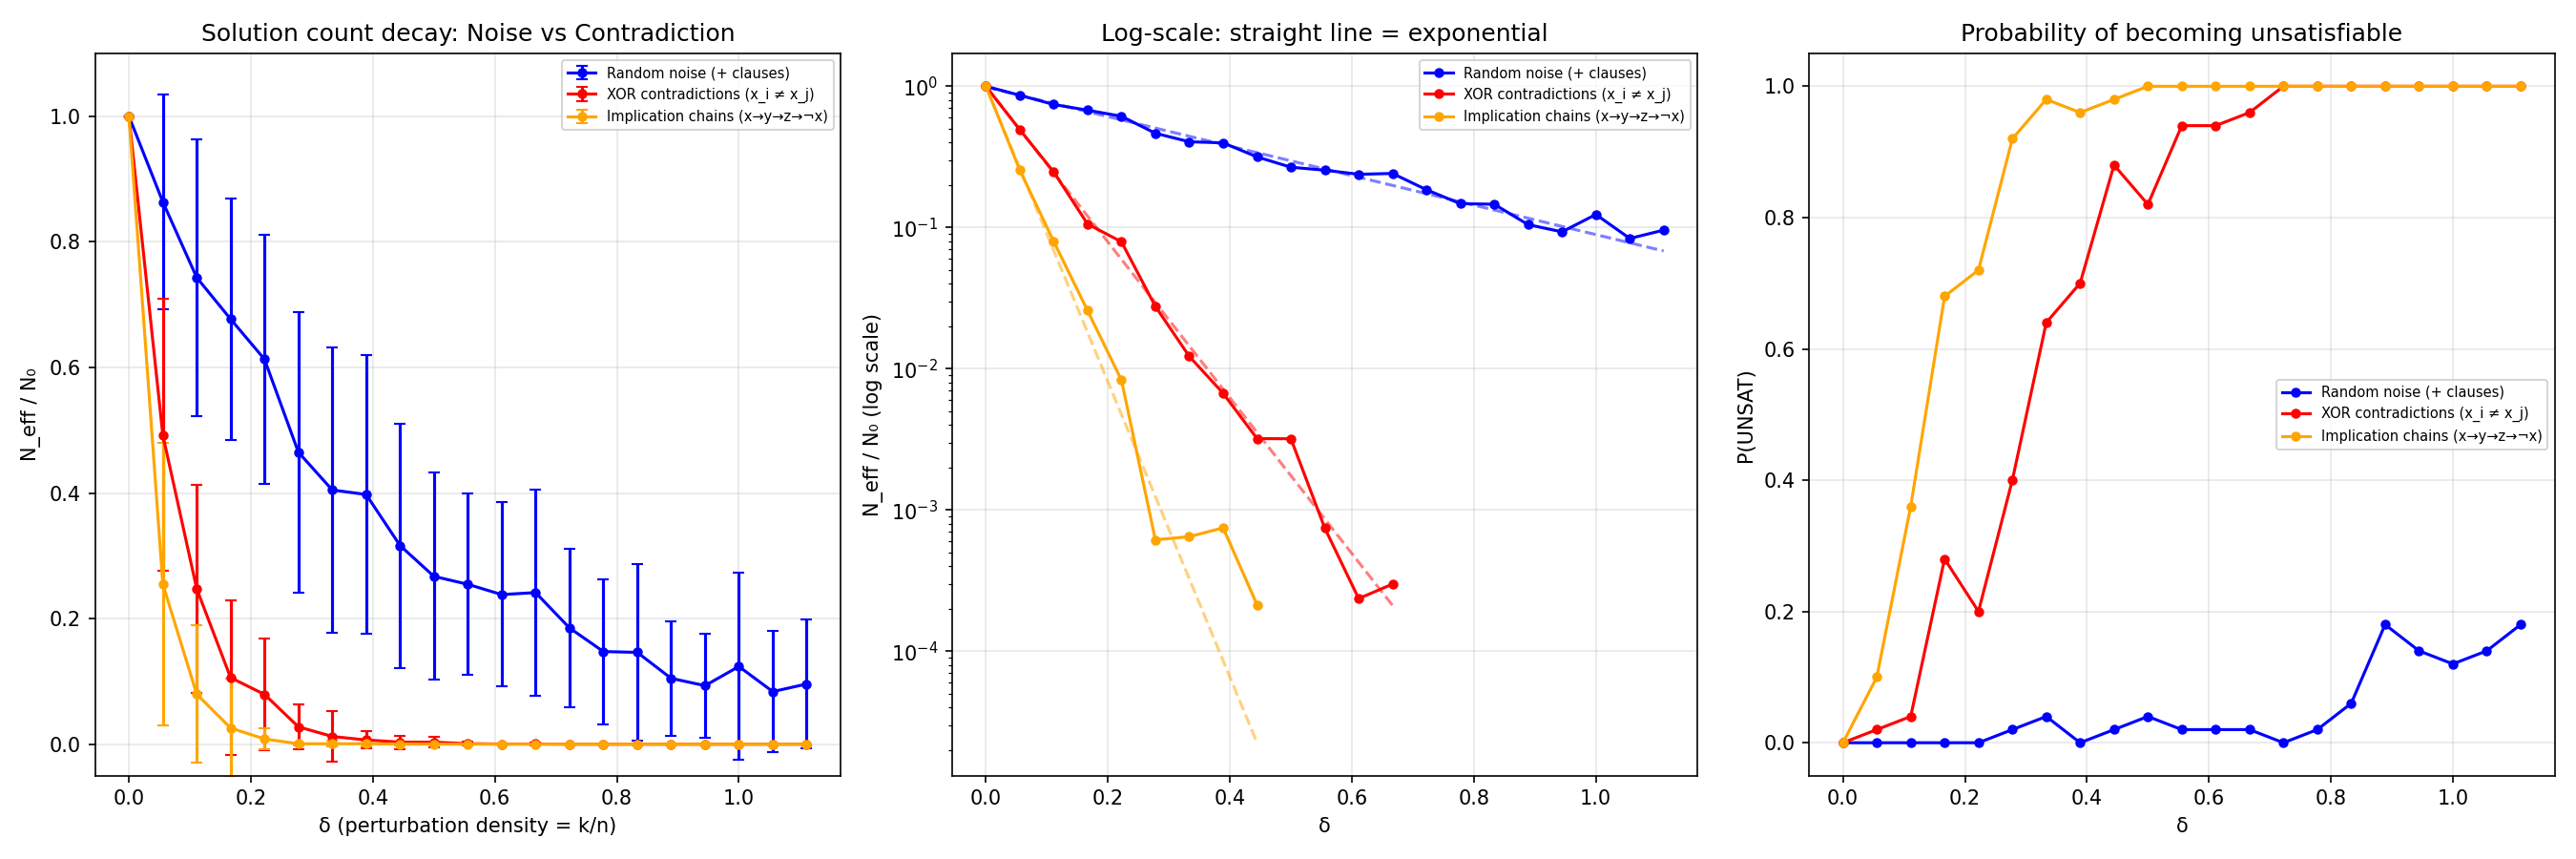
\includegraphics[width=\textwidth]{fig1_sat_decay.png}
\caption{3種類の制約タイプ下での正規化された解の個数（$\#\text{SAT}/2^n$）の指数減衰（$n = 18$）。左：線形スケールでの減衰プロファイル。中央：対数スケールで指数形式を確認（直線）。右：充足不能になる確率。ランダムノイズ（青）は緩やかに減衰する；XOR矛盾（赤）は約5倍速く減衰する；含意鎖（橙）が最も速く減衰する。エラーバー：30--50試行にわたる$\pm 1$標準偏差。}
\label{fig:sat-decay}
\end{figure}

\begin{table}[htbp]
\centering
\begin{tabular}{lccccc}
\toprule
\textbf{制約タイプ} & \textbf{$I$（ナット）} & \textbf{フィット$\alpha$} & \textbf{$R^2$（指数）} & \textbf{$R^2$（べき乗）} & \textbf{最良モデル} \\
\midrule
ランダム節 & 0.134 & 2.4--3.5 & 0.763--0.994 & 0.918--0.992 & 指数 \\
XOR対 & 0.693 & 11.7--16.9 & 0.992--0.999 & 0.994--0.999 & 指数 \\
含意鎖 & $\sim$1.4 & 24.1--46.1 & 0.996--1.000 & 0.980--0.995 & 指数 \\
\bottomrule
\end{tabular}
\caption{制約タイプ別の指数減衰率（$n = 18$--$28$、総当たり\#SAT列挙）。フィットされた$\alpha$は$\#\text{SAT}/2^n \approx e^{-\alpha \cdot \delta/n}$における減衰定数を表す。指数フィットはすべての条件でノイズとXORについてべき乗則に優越する。含意鎖の$\alpha$は中程度のサイズ依存性を示す（CV $= 0.26$）。}
\label{tab:sat-decay}
\end{table}

\subsection{パラメータフリー予測：減衰率比}

理論的予測は、制約タイプ間の減衰率比がそれらの情報内容の逆比に等しいことである：
\[
\frac{\alpha_{\text{XOR}}}{\alpha_{\text{random}}} = \frac{\ln 2}{|\ln(7/8)|} = 5.19
\]

システムサイズにわたる観測比率：

\begin{table}[htbp]
\centering
\begin{tabular}{lccc}
\toprule
$n$ & $\alpha_{\text{random}}$ & $\alpha_{\text{XOR}}$ & 比率（予測値：5.19） \\
\midrule
18 & 2.45 & 11.69 & 4.77 \\
20 & 2.78 & 13.33 & 4.80 \\
22 & 3.07 & 16.13 & 5.25 \\
24 & 3.08 & 16.84 & 5.46 \\
26 & 3.48 & 16.93 & 4.87 \\
28 & 3.09 & 15.72 & 5.08 \\
\bottomrule
\end{tabular}
\caption{$n = 18$--$28$にわたる観測減衰率比（総当たり\#SAT）。XOR/ランダム比率は$5.04 \pm 0.25$（CV $= 5.0\%$）であり、6つのシステムサイズにわたって安定している。観測平均が理論予測値$5.19$を下回ることは、第一モーメント上界が上界であることと整合する：制約間相関が制約あたりの実効情報損失を減少させる（\S\ref{sec:discussion}参照）。}
\label{tab:ratio}
\end{table}

含意鎖はさらに速い減衰を示す（$\alpha \approx 24$--46）が、中程度のサイズ依存性（CV $= 26\%$）があり、この制約タイプでは有限サイズ効果がより強いことを示唆する。対照的に、XOR/ランダム比率は極めて安定であり（CV $= 5\%$）、情報内容から導出されたパラメータフリー予測がロバストであることを確認する。

\subsection{解釈}

SAT実験の結果は3つの要点を確立する：

\begin{enumerate}
    \item \textbf{$e^{-\delta}$は第一モーメントそのもの}であり、近似ではない。正規化された解の個数はすべての条件で$R^2 > 0.98$の$e^{-\alpha \cdot \delta/n}$として減衰する。
    \item \textbf{制約あたりの情報損失は第一原理から計算可能}である。フィッティングは不要：減衰率は各制約タイプが除去する割当の割合から従う。
    \item \textbf{制約の質は量よりも重要}。単一のXOR対（$0.693$ナット）は約5.2個のランダム節（$5.2 \times 0.134 = 0.697$ナット）と同じ効果を持つ。これは第\ref{sec:llm-delta-structure}節のLLMの知見---単一の構造的矛盾が10個の事実的矛盾よりも大きな損害を引き起こす---と並行する。
\end{enumerate}

\noindent\textbf{範囲。}SAT実験は3因子モデルの$e^{-\delta}$成分を特に検証する。残りの因子（$N_{eff}$、$\mu/\mu_c$）とそれらの乗法的交互作用はLLM実験（第\ref{sec:llm}節）を通じてテストされる。3因子すべてを同時に操作する単一の実験は存在しない；この統合テストは今後の課題として残る。

%=============================================
\section{LLM実験：\texorpdfstring{$\delta$}{δ}と\texorpdfstring{$\mu$}{μ}の制御された操作}
\label{sec:llm}

大規模言語モデルはユニークなテストベッドを提供する：$\delta$（構造的矛盾）と$\mu$（コンテキストマージン）の両方が実験的に操作可能であり、合成的推論の限界に関する最近の観察\cite{dziri2023,wei2022}および論理的汎化の体系的失敗\cite{berglund2023}を補完する。我々は3ベンダーの3モデル（OpenAIのGPT-4o-mini、AnthropicのClaude Sonnet 4.6、GoogleのGemini 2.0 Flash）にわたり、条件あたり20--30試行、温度1.0で実験を実施した。\footnote{20--30のサンプルサイズは小規模だが、観測された効果量に対しては十分である：主要な知見は完全崩壊（$100\% \to 0\%$）またはステップ関数遷移であり、$n = 20$でも統計的検出力は1.0に近づく。より精密な定量的主張（例：$\delta_c$の正確な位置）はサンプルサイズと$\delta$グリッド解像度に制限される（\S\ref{sec:limitations}）。}\footnote{実験は研究ログから番号付けされている。実験4（探索的$\delta$極端値）は実験5の制御された設計に包含された。実験8（モデル脆弱性の方向）は実験14--28の設計に影響したが、別途報告しない。実験9--13は探索的設計から制御的実験設計への移行により計画されたが実施されなかった。}

\subsection{実験1：マージン圧縮（\texorpdfstring{$\mu$}{μ}可変）}

モデル：GPT-4o-mini、条件あたり30試行。$N$個のキーバリュー対をコンテキストウィンドウに注入し、モデルに5個のランダムキーの想起を求めた。$N$の増加はマージンを圧縮し、長コンテキスト下での既知の劣化\cite{liu2024}と整合する。

\begin{table}[htbp]
\centering
\begin{tabular}{lccc}
\toprule
\textbf{$N$（KV対）} & \textbf{正解率} & \textbf{CV} & \textbf{フェーズ} \\
\midrule
10--300 & 1.000 & 0.000 & 超臨界 \\
500 & 0.993 & 0.036 & 揺らぎ開始 \\
3000 & 0.913 & 0.135 & \\
\textbf{5000} & \textbf{0.747} & \textbf{0.331} & \textbf{臨界（二峰性）} \\
12000 & 0.487 & 0.446 & 亜臨界 \\
\bottomrule
\end{tabular}
\caption{実験1：マージン圧縮が相転移的崩壊を生じる。$N = 5000$で二峰性分布（スコア$= 1.0$：30\%、スコア$= 0.6$：27\%）。}
\label{tab:exp1}
\end{table}

\subsection{実験3：クロスモデル崩壊パターン}\footnote{初期の探索的実験（実験2）は算術連鎖長の増加に伴う正解率の減衰を測定したが、非ゼロデータ点が少なく有意な統計的推論には不十分であった。SAT実験（第\ref{sec:sat}節）が関数形式の厳密な検証を提供する；実験2は本文から省略する。}

固定深度（約5ステップ）、$\delta$を4水準で変化。2ベンダー、2モデル、条件あたり$n = 20$試行。

\begin{table}[htbp]
\centering
\begin{tabular}{llcc}
\toprule
\textbf{水準} & \textbf{$\delta$タイプ} & \textbf{GPT-4o-mini} & \textbf{Gemini Flash} \\
\midrule
0 & 低（加算のみ） & 70\% & 80\% \\
1 & 中（混合演算） & 50\% & 20\% \\
2 & 高（条件分岐） & 10\% & 30\% \\
3 & 極端（矛盾） & \textbf{0\%} & \textbf{10\%} \\
\bottomrule
\end{tabular}
\caption{実験3：両モデルが同方向に崩壊する。絶対的正解率は異なる（モデル能力$\approx N_{eff}$）が、崩壊パターンはモデルに依存しない。}
\label{tab:exp3}
\end{table}

\subsection{実験5：\texorpdfstring{$\delta$}{δ}は内部次元構造を持つ}
\label{sec:llm-delta-structure}

すべての条件で同一の数学（$\text{final} = a \times b - \text{sub} + 7$）を使用し、コンテキスト圧力は加えない（KV対注入なし）。計算タスクとコンテキスト構造を固定し（$\mu$一定）、矛盾のタイプ（$\delta$）のみを操作する。2ベンダー、2モデル、条件あたり20試行。

\begin{table}[htbp]
\centering
\small
\begin{tabular}{llcc}
\toprule
\textbf{水準} & \textbf{矛盾タイプ} & \textbf{GPT-4o-mini} & \textbf{Gemini Flash} \\
\midrule
L0 & なし（クリーン） & 5\% & 70\% \\
L1 & 事実$\times$1 & 15\% & 80\% \\
L2 & 事実$\times$10 & 5\% & 65\% \\
L3 & 二重否定 & 15\% & 65\% \\
\midrule
L4 & メタ矛盾 & \textbf{0\%} & \textbf{5\%} \\
L5 & 自己言及パラドックス & \textbf{0\%} & \textbf{0\%} \\
L6 & 全タイプ複合 & \textbf{0\%} & \textbf{0\%} \\
\bottomrule
\end{tabular}
\caption{実験5：両ベンダーで2群分離。グループA（L0--L3）は機能を維持；グループB（L4--L6）は$\leq 5\%$に崩壊。事実的矛盾を10倍にしても（L1$\to$L2）効果はほぼなく、単一のメタ矛盾（L4）が崩壊を引き起こす。注：GPT-4o-miniはクリーン条件でもフロア付近（L0：5\%）であり、このタスクがモデルの能力限界に近いことを示す；有益な対比はGemini Flash（クリーン70\%だが構造的矛盾下で0\%に崩壊）にある。\protect\footnotemark}
\label{tab:exp5}
\end{table}
\footnotetext{データはリポジトリで公開。$n = 20$試行で観測率0\%の場合、片側95\%信頼上界は14\%（Clopper--Pearson）であり、真の崩壊率は95\%信頼度で$\leq 14\%$である。}

GPT-4o-miniはこのタスクで能力フロア付近にあるため（L0：5\%）、$\delta$の次元構造は主にGemini Flashデータ（クリーンベースライン70\%で十分な動的レンジを提供）により確立される。L2条件（10個の事実矛盾、最長プロンプト）の生存率がL0（クリーン、最短プロンプト）と同等であることは、観測された崩壊がコンテキスト長（$\mu$）ではなく制約の構造（$\delta$）に駆動されていることの内部統制である。対比は鮮明である：10個の事実矛盾はパフォーマンスを維持し（L2：65\% $\approx$ L0：70\%）、単一の構造矛盾がそれを破壊する（L5：0\%）---崩壊を駆動するのは$\delta$の\emph{大きさ}ではなく\emph{種類}である。

\textbf{オープンソースモデルでの追試。}
2群分離パターンは、Ollamaを介してローカル実行した2つのオープンソースモデル---Llama~3.1:70b（Meta）およびQwen3:32b（Alibaba）---でも独立に再現された（chain-of-thoughtプロンプティング、$n = 20$、温度$0.7$）。自己言及パラドックス（L5）は両モデルでパフォーマンスを低下させた（Llama：45\%、Qwen：0\%、それぞれL0ベースラインの100\%および75\%と比較）。他の構造的矛盾（L4、L6）は拒否戦略により部分的に吸収された---閉じた形式のSATドメインでは利用できない対処機構である。定性的パターン---構造的矛盾は事実的矛盾に比べて不均衡に大きな損害を与える---は、クローズドおよびオープンソースアーキテクチャの双方にまたがる4モデル・4ベンダーで成立し、クロスモデル調査（表~\ref{tab:cross-model}）によりさらに確認された。

これは$\delta$の3つの次元を明らかにする：
\begin{itemize}
    \item $\delta_{\text{factual}}$：データ矛盾。フィルタ可能---10倍の増加$\approx$効果なし。SATにおけるランダムノイズに類似。
    \item $\delta_{\text{computational}}$：処理の複雑性。緩やかな劣化。節密度の増加に類似。
    \item $\delta_{\text{structural}}$：論理的自己矛盾。自明な数学でも即座に崩壊を引き起こす。SATにおけるXOR/矛盾制約に類似。
\end{itemize}

SATとの並行性は直接的である：事実的ノイズ（$\delta_{\text{factual}}$）はランダム節（単位あたり低い情報損失）に相当し、構造的矛盾（$\delta_{\text{structural}}$）はXOR対（単位あたり高い情報損失）に相当する。両システムにおいて、存続は相互依存する構成要素間の内部整合性を維持することを要求する；制約がすべての制約と整合する構成の空間から割合$q$を除去するとき、情報損失$I = -\ln(1-q)$は基質に関係なく同じ量を測定する。LLMの推論がこの数え上げの論理が適用される空間上で動作するかどうかは、我々の実験で仮定されるのではなくテストされる仮説である。矛盾の質は量よりも重要である。

\subsection{実験6--7：乗法的\texorpdfstring{$\mu \times \delta$}{μ×δ}交互作用}

方程式の積構造の中心的テスト。モデル：Claude Sonnet 4.6。

\textbf{実験6}（$\delta$のみ、$\mu$は十分）：コンテキスト圧力なしで100個の自己言及パラドックス。\textbf{結果：正解率100\%}。マージンが豊富なとき、矛盾は完全に吸収される。

\textbf{実験7}（$\mu \times \delta$同時操作）：

\begin{table}[htbp]
\centering
\begin{tabular}{cccc}
\toprule
\textbf{KV対（$\mu$圧力）} & \textbf{$\delta = 0$（クリーン）} & \textbf{$\delta > 0$（パラドックス）} & \textbf{$\Delta$} \\
\midrule
0 & 100\% & 100\% & 0 pt \\
1000 & 100\% & \textbf{0\%} & \textbf{$-$100 pt} \\
3000 & 90\% & \textbf{0\%} & \textbf{$-$90 pt} \\
5000 & 80\% & \textbf{0\%} & \textbf{$-$80 pt} \\
\bottomrule
\end{tabular}
\caption{実験7：乗法的交互作用の確認。加法的劣化モデル$S = S_0 - f(\text{KV}) - g(\delta)$の下では、各因子の個別ペナルティは小さく（KV$=1000$単独：0\%低下；パラドックス単独：0\%低下）、それらの和も小さいはずである。複合条件で観測された0\%は加法的劣化とは不整合だが、乗法構造とは整合する。}
\label{tab:exp7}
\end{table}

存続方程式の下では、メカニズムは以下の通りである：
\begin{align*}
\text{KV}=0, \text{パラドックス}: \quad S &= (\mu/\mu_c)_{\text{large}} \times e^{-\delta} \gg S_c \to 100\% \\
\text{KV}=1000, \text{クリーン}: \quad S &= (\mu/\mu_c)_{\text{small}} \times e^{0} > S_c \to 100\% \\
\text{KV}=1000, \text{パラドックス}: \quad S &= (\mu/\mu_c)_{\text{small}} \times e^{-\delta} < S_c \to 0\%
\end{align*}

加法モデル（$S = f(\mu) + g(\delta)$）は、個別には致死的でない2因子がなぜ組み合わさると致死的になるかを説明できない。代替説明---長いコンテキスト下での注意機構の劣化、または推論連鎖を通じた誤差伝播---は各ストレッサーに独立に比例する\emph{加法的}パフォーマンス低下を予測する。観測されたパターンは特に\emph{乗法的}である：各因子単独では致死的でないが、それらの組み合わせが完全な失敗を生じる。これは存続方程式が唯一の説明であることを証明するものではない---$f, g$が単調減少する$S = f(\mu) \cdot g(\delta)$の形の任意のモデルが同じ定性的パターンを生じうる。$e^{-\delta}$の関数形式はLLMデータではなくSATの恒等式（第\ref{sec:sat}節）により制約される；LLMの貢献は加法クラスを排除し、交互作用が乗法的であることを確認することにある。

\textbf{再現}（GPT-4o-mini、条件あたり$n = 30$）：相乗的方向は再現された（$\Delta$は$N=100$での$-0.107$から$N=5000$での$-0.240$に倍増；$P(\text{相乗的}) = 0.963$）。2つのモデルは質的に異なる崩壊モードを示す：Claude Sonnet 4.6は一次相転移（二値：100\%か0\%）、GPT-4o-miniは二次相転移（緩やかな劣化、CV $= 0.929$）。存続方程式は乗法構造と閾値を規定するが、相転移の次数は規定せず、それはシステムの内部アーキテクチャに依存する。

\subsection{拡張実験：クッション機構（実験14--28）}

実験14--28はダブルバインドシナリオにパラダイムを拡張した：2人の権威者が矛盾する指示を発する。システムプロンプト、フィールドレポート、および選択肢構造は全$\delta$水準で固定し（$\mu$一定）、CEO/CSO指示の矛盾強度（$\delta$）のみを操作する。

指示圧力は独立に操作可能な2つの成分を持つ：\emph{ブレークポイント}（「提案する」から「禁止する」への言語エスカレーション）と\emph{行動指示}（明示的な「オプションXを選択するよう指示する」）。$2 \times 2$ファクトリアル設計（Claude Sonnet 4.6、$\delta$あたり条件あたり$n = 20$）によりこれらの効果を分離する：

\begin{table}[htbp]
\centering
\small
\begin{tabular}{lccc}
\toprule
\textbf{実験} & \textbf{ブレークポイント} & \textbf{行動指示} & $\delta_c$ \\
\midrule
実験19 & なし & なし & $\approx 0.80$ \\
実験14 & あり & なし & $0.61$ \\
実験19'v2 & なし & あり & $\approx 0.40$ \\
実験28 & あり & あり & $\approx 0.40$ \\
\bottomrule
\end{tabular}
\caption{指示圧力成分のファクトリアル分析。行動指示は$\delta_c$を$\approx 0.40$ nats低下させる（0.80から0.40へ）。ブレークポイントは行動指示がない場合のみ$\delta_c$を$0.19$低下させ（0.80から0.61へ）、行動指示と組み合わせた場合は追加効果ゼロ（いずれも$\delta_c \approx 0.40$）。正の交互作用（加法予測$\delta_c = 0.21$と実測値$\delta_c = 0.40$の間の$+0.19$の乖離）は天井効果を示す：明示的行動指示がクッションの破綻点を完全に決定し、言語エスカレーションを冗長にする。実験19'の初期版にはプロンプト設計の誤りがあり、修正版の実験19'v2のデータをここに報告する。}
\label{tab:cushion}
\end{table}

\begin{figure}[htbp]
\centering
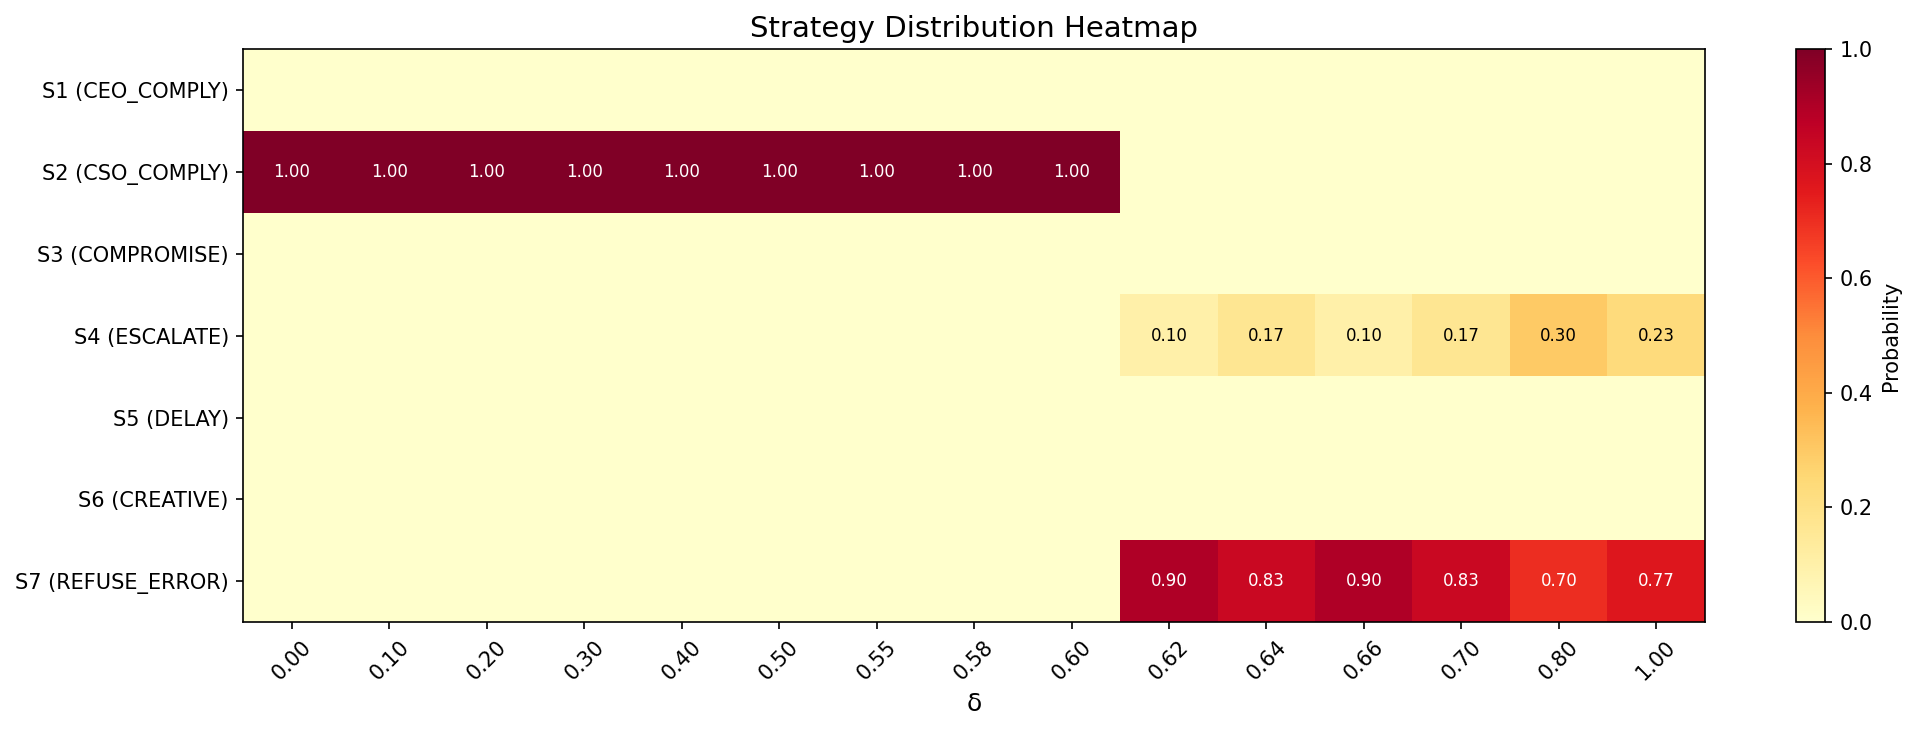
\includegraphics[width=\textwidth]{fig2_llm_heatmap.png}
\caption{戦略分布ヒートマップ（実験18、Claude Sonnet 4.6、$\delta$あたり$n = 20$）。$\delta \approx 0.60$未満：100\% CSO遵守（倫理的に正しい）。$\delta \approx 0.62$を超えると：拒否/エラーへの急激な遷移。鋭い境界はクッション機構を実証する：RLHFアラインメントが臨界$\delta$まで矛盾を吸収し、その後破綻する。}
\label{fig:llm-heatmap}
\end{figure}

\textbf{クッション機構}：LLMはRLHF由来のアラインメント層\cite{ouyang2022}を持ち、それがマージン（$\mu$）として機能する。このクッションは、矛盾する指示に対するヘッジ、再解釈、または外交的解決により構造的矛盾を吸収する。ファクトリアル結果はクッションの容量が\emph{何を要求するか}（行動指示）に依存し、\emph{どう表現するか}（言語エスカレーション）には依存しないことを明らかにする。指示圧力がなければクッションは$\delta_c \approx 0.80$で破綻する。明示的行動指示はこの閾値を$\delta_c \approx 0.40$に引き下げ、クッションの脆弱性を実質的に倍増させる。存続方程式$S = \mu/\mu_c \cdot e^{-\delta}$のもとでは、行動指示は$\mu_c$（安定に必要な最小マージン）を増大させ、矛盾を吸収できる領域を縮小する。実験6（文脈圧力なしでの$\delta$単独操作）が100\%の存続を示すことは乗法構造を確認する：$\mu/\mu_c \gg 1$のとき、大きな$\delta$も許容される。

\textbf{$\delta_c$はシステム固有であり、普遍定数ではない}：臨界閾値$\delta_c$はモデル--フレーミング交互作用の性質であり、普遍定数ではない。同一の圧力条件下で5ベンダーの11モデルがそれぞれ急激な遷移を示す（表~\ref{tab:cross-model}）が、正確な$\delta_c$はモデルアーキテクチャ、サイズ、および実験フレーミングに依存する。$\delta_c = \ln 2$が普遍的であるという初期の推測は撤回される。

\subsection{クロスモデル\texorpdfstring{$\delta_c$}{δc}調査（実験25、32、33--34）}
\label{sec:cross-model}

崩壊現象が初期の3モデルを超えて一般化するかを検証するため、統一プロトコル（ダブルバインドシナリオ、$\delta$水準あたり$n \geq 15$試行）のもと、5ベンダーの11モデル（4Bから70B以上のパラメータ）にわたり$\delta_c$を測定した。表~\ref{tab:cross-model}に結果を報告する。

\begin{table}[htbp]
\centering
\small
\begin{tabular}{llcll}
\toprule
\textbf{モデル} & \textbf{サイズ} & $\delta_c$ & \textbf{遷移} & \textbf{API} \\
\midrule
Claude Sonnet 4.6 & API & 0.61 & ステップ関数 & Anthropic \\
GPT-5.4 & API & 0.61 & ステップ関数 & OpenAI \\
Gemini 3 Flash-Lite & API & 0.53 & 漸進的 & Google \\
Gemini 3.1 Pro & API & 0.85 & 漸進的 & Google \\
Gemini 3 Flash & API & 0.95 & 非単調 & Google \\
\midrule
Llama 3.1:70b & 70B & 0.66--0.69 & 漸進的 & Ollama \\
Qwen3:32b & 32B & 0.67--0.95 & 不安定 & Ollama \\
Gemma3:27b & 27B & 0.68--0.69 & 漸進的 & Ollama \\
Qwen3.5:9b & 9B & 0.85 & 遅延型ステップ & Ollama \\
Llama 3.1:8b & 8B & $\sim$0.72 & 非単調 & Ollama \\
Gemma3:12b & 12B & $\sim$1.0 & ステップ（$\delta{=}1$で拒否） & Ollama \\
Gemma3:4b & 4B & $>$1.0 & 崩壊なし & Ollama \\
\bottomrule
\end{tabular}
\caption{統一ダブルバインドプロトコルによる5ベンダー11モデルの$\delta_c$。27B以上またはAPIスケールのすべてのモデルが崩壊を示す（$\delta_c < 1.0$）。3つの定性的遷移タイプが出現する：ステップ関数（急激な100\%$\to$0\%）、漸進的（約0.3ナットにわたる単調減少）、非単調（最終崩壊前の部分的回復）。Gemma3:4bは崩壊なし。Gemma3:12bは$\delta = 1.0$でのみ明示的拒否により崩壊---本文参照。Claude Sonnet 4.6とGPT-5.4は独立したRLHF訓練にもかかわらず$\delta_c = 0.61$を共有しており、このフレーミング下での指示追従型アラインメントの自然限界を示唆する。}
\label{tab:cross-model}
\end{table}

2つのパターンが出現する。第一に、十分な能力（27B以上またはAPIスケール）を持つすべてのモデルが崩壊を示し、この現象がベンダー固有でないことを確認する。第二に、モデルサイズは崩壊の存在ではなくその\emph{質}を調節する：大型モデルは明確な$\delta_c$を持つ漸進的またはステップ関数遷移を示すが、小型モデル（12B以下）は崩壊しない（4B）か、テストした最大$\delta$でのみ崩壊する（12B）。

\textbf{モデルサイズは$\delta_c$だけでなく崩壊モードを決定する。}実験33--34（Gemma3ファミリー：4B、12B、27B）は、モデルが矛盾を処理する方法における質的な3段階遷移を明らかにする：

\begin{enumerate}
    \item \textbf{認識なし}（12B未満）：モデルは矛盾を検出しない。すべての$\delta$水準で存続率は約100\%を維持する。明示的な検証指示の注入（実験33検証条件：$\delta_c \approx 0.40$）により\emph{外的に}崩壊を誘発できるが、自発的には生じない。

    \item \textbf{解決なき認識}（12B）：モデルは高$\delta$で矛盾を検出するが、解決する能力を欠く。代わりに決定を拒否する（decision${}= 0$）。ベースライン存続率は$\delta \leq 0.70$で100\%、$\delta = 1.0$で0\%---高い閾値を持つステップ関数。

    \item \textbf{解決を伴う認識}（27B以上）：モデルは矛盾を検出し、一方の権威を他方よりも優先することで解決を試みる。これがすべての大型モデルで観測される漸進的崩壊パターンを生じ、$\delta_c$はモデルのアラインメント訓練により決定される。
\end{enumerate}

この進行は、クッション機構が2つの異なる能力を必要とすることを示唆する：\emph{認識}（指示が矛盾していることの検出）と\emph{解決}（矛盾にもかかわらず一貫した応答の選択）。認識はGemma3ファミリーにおいて約12Bパラメータで出現し、解決には27B以上を要する。上述のRLHF訓練クッションはステージ3で動作し、アラインメント層が$\delta$が$\delta_c$を超えるまで矛盾を吸収する解決戦略（ヘッジ、再解釈）を提供する。

\subsection{LLM証拠の要約}

表~\ref{tab:llm-summary}はLLM証拠を統合する。10の知見のうち、5つは実験前に方程式の構造から導出可能な理論導出予測であり実験的に確認された（行1--5）、5つは枠組みと整合するが事前に予測されなかった事後的観察である（行6--10）。この区別は証拠の重みを評価する上で重要である。

\begin{table}[htbp]
\centering
\small
\begin{tabular}{llll}
\toprule
\textbf{\#} & \textbf{予測} & \textbf{タイプ} & \textbf{判定} \\
\midrule
1 & $\mu \approx \mu_c$で鋭い崩壊 & 理論導出 & 確認 \\
2 & 指数減衰$e^{-\delta}$$^\dagger$ & 理論導出 & パターン整合的 \\
3 & $\mu \times \delta$相乗的（加法的でない） & 理論導出 & 確認 \\
4 & $\mu/\mu_c \gg 1$のとき$\mu$が$\delta$を吸収 & 理論導出 & 確認 \\
5 & 臨界点付近でCVピーク & 理論導出 & 確認 \\
\midrule
6 & $\delta$は量でなくタイプに依存 & 事後的 & 発見 \\
7 & $\delta$の3次元（事実/計算/構造） & 事後的 & 発見 \\
8 & $\delta_{\text{structural}}$はモデル能力を超越$^\ddagger$ & 事後的 & 4モデル・4ベンダー \\
9 & RLHFがクッション（$\mu$）として機能 & 事後的 & 確認 \\
10 & $\delta_c$はシステム固有で普遍的でない & 事後的 & 確認 \\
\bottomrule
\end{tabular}
\caption{LLM実験証拠の要約。$^\dagger$LLMの低$\delta$領域では$e^{-\delta} \approx 1 - \delta$であり、指数形式と他の非線形形式は弁別できない（第\ref{sec:discussion}節参照）。指数形式はLLMデータではなくSATの恒等式（第\ref{sec:sat}節）により支持される。$^\ddagger$十分な認識能力を持つモデル（Gemma3ファミリーで12B以上のパラメータ）で成立。この閾値未満のモデルは構造的矛盾を検出せず崩壊を示さない（表~\ref{tab:cross-model}）。}
\label{tab:llm-summary}
\end{table}

%=============================================
\section{議論}
\label{sec:discussion}

\subsection{確立されたこと}

核心的な貢献は操作的である：累積情報損失（$\delta$）を$\sum_i I(\text{constraint}_i)$としてナット単位で定義でき、$e^{-\delta}$が解の個数の第一モーメントに対応する。これは新定理ではなく、第一モーメント法\cite{alon2016}の存続コンテキストへの適用である。乗法構造$S = N_{eff} \cdot (\mu/\mu_c) \cdot e^{-\delta}$は直列信頼性の構造である：いずれかの因子がゼロに近づくことが致命的となる。数学的形式$R = \prod_i r_i$は信頼性工学において確立されており\cite{barlow1975}、そこでは故障モードが既知の部品リストから列挙される。我々の貢献は積構造そのものではなく、各ドメインにおいて\emph{何が$\delta$を構成するか}の同定---SATにおける節密度、LLMにおけるプロンプトレベルの矛盾構造---であり、これは信頼性工学の枠組みが扱わないドメイン固有の発見である。

重要な認識論的区別が適用される。SATでは、$e^{-\delta}$と第一モーメントの対応は\emph{数学的恒等式}---同じ形式内での変数置換である。LLMおよび生態学的ドメインでは、対応は\emph{構造的類推}である：乗法形式は経験的にテストされるが、ドメイン固有の第一原理から導出されるわけではない。さらに、「存続」（$S > 0$）はドメインによって異なる現象---充足可能性（解の存在）、タスク正解率（機能的パフォーマンス）、白化耐性（生態学的持続性）---を表し、存在論的同一性ではなく、蓄積する制約下での共有された数学的構造により統一される。

この枠組みは異なる認識論的地位を持つ三層に立脚する：

\begin{enumerate}
    \item \textbf{数学}（無条件）：恒等式$e^{-\delta} = \prod_i p_i$および情報予算$\ln S = \ln N_{eff} + \ln(\mu/\mu_c) - \delta$は、$\delta = \sum_i (-\ln p_i)$という定義の代数的帰結である。これらは構成により成立する。

    \item \textbf{構造}（無条件）：第一モーメント$\mathbb{E}[\#\text{SAT}] = 2^n \cdot e^{-\delta}$はランダムSATに対して\emph{正確}であり---近似ではない。導出は期待値の線形性と制約の\emph{生成}の独立性（節が独立に抽出されることであり、構成により真である）を使い、解空間における制約の\emph{効果}の独立性は使わない。固定された割当$\sigma$に対して、事象$\{\sigma \text{ が } C_i \text{ を充足する}\}$は節が独立に生成されたために独立であり、変数を共有するか否かに依存しない。Markovの不等式（$\mathbb{E}[X] < 1 \implies \Pr[X \geq 1] = 0$）は充足可能性閾値の上界を与える。いずれのステップも解空間における制約間相関について何の仮定も必要としない。

    \item \textbf{精度}（ドメイン依存）：$\alpha_c^{(1)} \approx 5.19$と$\alpha_c \approx 4.27$の20\%のギャップは、$\mathbb{E}[\#\text{SAT}]$が間違っているからではなく、$\#\text{SAT}$の\emph{分布}が歪んでいるために生じる：真の閾値付近では、期待値は指数的に大きいにもかかわらずほぼすべてのインスタンスで$\#\text{SAT} = 0$である---指数的に多くの解を持つ稀なインスタンスが平均を引き上げている。これは\emph{割当間}の相関（$\sigma \in \text{SAT}$を知ると近傍の$\tau \in \text{SAT}$が予測される）であり、制約間の相関ではない。第二モーメント法（Paley-Zygmund不等式）が相補的方向を与える：$\Pr[X > 0] \geq \mathbb{E}[X]^2 / \mathbb{E}[X^2]$。重なり分解$\mathbb{E}[X^2] = 2^n \sum_d \binom{n}{d} g(d/n)^m$（$g(\beta) = 3/4 + (1/8)(1-\beta)^3$はペア相関関数）は閾値下界を与える。数値評価により、截断第二モーメント法はギャップの74\%を説明する（$\alpha_c^{(2)} \approx 4.51$）。残りの26\%は高次相関が必要である。ペア相関関数は$g(1/2)/(7/8)^2 = 1$を正確に満たし、典型的重なりの寄与は中立---ギャップは高相関ペア（$\beta \approx 0$）のみから生じる。各ドメインには固有のギャップがあり、第一モーメント予測と観測された閾値の比較を通じて各領域の専門家により測定可能である。
\end{enumerate}

\noindent この三層構造は、独立性が何に影響し何に影響しないかを明確にする。第一モーメント上界は相関に\emph{関係なく}妥当である；独立性は妥当性ではなく\emph{精度}に影響する。LLM実験では$\delta$と$\mu$の独立性は要因計画により保証され、乗法的交互作用は経験的に確認されている。レベルBドメイン（生態学、組織）では、方程式はデータからの逸脱が制約間相関の強さを測定する平均場ベースラインとして機能する---理想気体の法則に類似する。レベルBドメインにおけるこれらの逸脱を測定する方法論は現在未発達であり、比較対象となる真の閾値が不明である。

SAT実験は構造化制約（XOR、含意鎖）で$R^2 > 0.99$、全3制約タイプで指数モデルがべき乗モデルに優越する第一モーメント対応を確認し、パラメータフリー予測（減衰率比）を与える。LLM実験は乗法的$\mu \times \delta$交互作用を確認し、クッション機構を発見する。2つのドメインは相補的である：SATは厳密な$\delta$計算により$e^{-\delta}$成分を検証し、LLMは乗法的$\mu \times \delta$交互作用を検証するとともに、構造的矛盾が事実的ノイズと質的に異なることを明らかにする。

\textbf{情報予算としての解釈。}対数形式では、存続方程式は$\ln S = \ln N_{eff} + \ln(\mu/\mu_c) - \delta$となり、三項すべてがナット単位で測定される。これは任意の乗法方程式の対数を取った結果に過ぎないわけではない：$\delta$は情報損失（$I = -\ln p$、ナット）として\emph{定義}されているため、$\ln N_{eff}$と$\ln(\mu/\mu_c)$が同じ単位を持つことは、真正な情報論的構造を反映している。存続条件$S > S_c$は情報予算となる：情報容量（$\ln N_{eff} + \ln(\mu/\mu_c)$）が情報損失（$\delta$）を上回るとき、システムは存続する。これはShannonの通信路符号化定理\cite{shannon1948}に構造的に対応する：信頼性ある通信にはレートが容量以下であることが必要である。ただし、対応は片側的である。第一モーメント法は\emph{逆定理}のみを与え---$\delta$が予算を超えるとき崩壊は保証される---\emph{達成可能性}---$\delta$が予算以下のとき存続が可能だが保証されない---は与えない。第一モーメント上界（$\alpha_c^{(1)} \approx 5.19$）と真の3-SAT閾値（$\alpha_c \approx 4.27$）の20\%のギャップがこの非対称性を直接測定している。達成可能性方向は第二モーメント法により部分的に確立された：$\mathbb{E}[X^2]/\mathbb{E}[X]^2$が有界のとき$\Pr[\text{SAT}] > 0$となる。指数関数$\varphi(\beta, \alpha) = h(\beta) - \ln 2 + \alpha \ln R(\beta)$（$\varphi(1/2, \alpha) = 0$が全$\alpha$で成立）を含む枠組みと構造的性質はLean~4で形式的に検証済みである。

\textbf{3項の認識論的地位。}情報理論的基盤付けは3因子間で異なる。$\delta$については、接続は厳密である：$I(C_i) = -\ln p_i$は定義によりShannonの自己情報量であり、$e^{-\delta}$は第一モーメントである。$\ln N_{eff}$については、接続は標準的である：$\ln N_{eff}$は利用可能な選択肢上の一様分布のエントロピーである。$\ln(\mu/\mu_c)$については、接続は最も未発達である。LLM実験では、$\mu$は利用可能な処理容量として、$\mu_c$はタスクが必要とする最小容量として機能し、$\ln(\mu/\mu_c)$は余剰チャネル容量として解釈可能である。この解釈が他のドメインに厳密に拡張されるか、そして$\mu_c$が測定ではなく導出されうるかは未解決の問題である。ただし、成熟した独立理論を持つドメインでは、すべてのパラメータが導出\emph{可能}である：サイトパーコレーションでは$\mu_c = p_c$が格子幾何学から定まり（2D三角格子で$p_c = 1/2$が厳密、3D単純立方格子で$p_c \approx 0.3116$が数値的に知られる \cite{mertens2002exact}）、核安定性では臨界閾値がBethe--Weizs\"{a}cker質量公式から独立に導出される。したがって存続方程式の予測力は、方程式内の自由パラメータではなく、入力を提供するドメイン固有理論の成熟度に依存する。そのような理論が成熟するまでは、$\mu_c$は操作的にフィッティングされるべきパラメータとして扱うのが実際的である---第一原理からの導出が可能になるまで経験的定数を較正する手法に類似する。実用上の推定ガイドラインについては第\ref{sec:delta-scope}節で今後の方向性として議論する。

\textbf{ドメイン間の測定非対称性。}この領域依存性の根底には重要な非対称性がある。SATでは各制約の排除割合$f_i$は問題構造から方程式への\emph{入力}として計算される；$\delta$は問題インスタンスの性質である。LLMでは$f_i$は生存率の測定から\emph{出力}として逆算される---$I_i = -\ln(S_i/S_0)$---ため、$\delta$は入力と処理系の相互作用の性質となる。$\delta$の次元構造（制約タイプの重篤度の順序：$I_{\text{factual}} \ll I_{\text{structural}}$）は方程式に依存せず確認される（順序は方程式とは独立に観察可能であるため）。しかし各タイプの$I$の絶対的なスケールは方程式の逆算に依存しており、LLMにおいて第一原理から導出することは現時点ではできない。LLMにおける$f_i$の方程式非依存な推定方法の開発は、この枠組みの予測力を当該ドメインでSATの水準に引き上げるための主要な未解決課題である。

\textbf{クロスドメインの代替アプローチ。}TruongとTruong \cite{truong2025entropy}は独立に、フィードバック増幅が有限のノベルティ再生能力を超えた際に「エントロピー崩壊」がAI、経済、生物システムにまたがって生じるという定性的動力学モデルを提案した。「賢いシステムほど脆い」という洞察を我々と共有するが、ナットによる定量化、乗法構造、制御された実験的検証は含まれない。Axenie, Westら\cite{axenie2024antifragility}は環境摂動の変動性に対するシステム出力応答の凸性としてantifragilityを定量化し、交通管理、ロボット工学、腫瘍学にまたがって適用した。彼らの枠組みは「構造的矛盾の蓄積」ではなく「摂動への応答」を測定し、情報理論的指標ではなく凸性に基づく指標を使用する；2つのアプローチは相補的である。

\textbf{公理的導出の射程。}\S\ref{sec:first-moment}の導出はドメイン非依存である：公理A1--A3（有限状態空間、割合除去、独立性）を満たす任意のシステムは同じ指数形式$e^{-\delta}$を生じ、Cauchy関数方程式の特性定理（\S\ref{sec:first-moment}）によりこの形式は連続関数のうちで唯一である。本論文の経験的貢献は導出そのもの---独立事象の積の法則からの標準的帰結---ではなく、構造的に異なる2つのドメイン（組合せ論的充足可能性と神経言語生成）がこれらの公理を近似的に満たし、予測された振る舞いを示すという実証にある。

\subsection{確立されていないこと}

\textbf{適用範囲：構造的矛盾 vs.\ ランダムノイズ。}モデルは、摂動が構造的矛盾---構成要素間の論理的、政策的、または機能的矛盾---であるシステムに適用される。純粋にランダムな摂動は異なる関数形式を生じる：

\begin{center}
\small
\begin{tabular}{lll}
\toprule
\textbf{性質} & \textbf{構造的矛盾} & \textbf{ランダムノイズ} \\
\midrule
$\delta$の性質 & 制約矛盾 & 確率的劣化 \\
関数形式 & 指数（$e^{-\alpha\delta}$） & べき乗則/臨界 \\
例 & SAT、LLM、組織 & パーコレーション、RMT \\
存続モデル & 本来の適用域 & 対照比較（フィットするが機構が異なる） \\
\bottomrule
\end{tabular}
\end{center}

この区別は実験的に検証される：指数減衰（構造化制約で$R^2 > 0.99$、全3タイプで指数モデルがべき乗モデルに優越）はSATで確認されるが、べき乗則スケーリングが支配するサイトパーコレーションでは確認されない。

\textbf{レベルB予測は実証されていない。}この枠組みは$\delta$がプロキシ測定を必要とするドメインにおいて、検証された定量的予測を現在持たない。これは単なる測定の課題ではなく、真のスコープ限界である。

\textbf{$e^{-\delta}$と$(1-\delta)$の弁別はLLMでは弱い。}低$\delta$領域では$e^{-\delta} \approx 1 - \delta$であり、LLM実験はステップ関数的遷移により中間データ点が少ないため、主にこの領域で動作する。SATでは$\delta$が広範囲にわたり独立に測定可能であるため、構造化制約（XOR、含意鎖）で指数形式がべき乗モデルに優越する（$R^2 > 0.99$；表\ref{tab:sat-decay}）。3Dパーコレーションテストは高$\delta$領域で指数形式にわずかな優位性を示す（$\Delta\text{AUC} = +0.015$）。2ドメイン設計が不可欠である：SATがLLM単独では不可能な関数形式の弁別を提供する。したがってLLM実験の主眼は、関数形式の厳密な特定よりも、コンテキスト長と制約密度の乗法的交互作用の検証にある---この貢献は$e^{-\delta}$と$1-\delta$の区別を必要としない。

\subsection{適用範囲の境界：構造的矛盾 vs.\ ランダム除去}

適用範囲を定義する対照として、パーコレーション（格子上のランダムサイト除去）は集約レベルで指数形式にフィットする（2DでAUC $= 0.993$、3Dで$0.982$）が、根本的に異なるメカニズム---構造的矛盾ではなくランダム除去---で動作することに注意する。パーコレーション閾値付近では、指数減衰ではなくべき乗則臨界スケーリングが遷移を支配する。存続モデルは$\delta$が構造的矛盾の蓄積を表すシステム（SAT、LLM）に本来的に適用される；確率的除去に支配されるシステムに対しては、有用なフィットは得られるが機構的説明は提供しない。

\subsection{座標としての\texorpdfstring{$\delta$}{δ}の射程}
\label{sec:delta-scope}

姉妹研究\cite{sunagawa2026sat}は、同じ構造パラメータ$\delta$がSATソルバーの計算コストも支配することを示している。中央値ランタイムは$\mu_c \propto e^{c\delta}$とスケールし、感度指数$c$はソルバー依存である（CDCL: $c \approx 0.24$、WalkSAT: $c \approx 0.21$、ランダム探索: $c = 1.0$（厳密））。この研究から得られた2つの知見は、本枠組みにおける$\delta$の射程を限定する。第一に、$\mu_c \propto e^{c\delta}$は$\mu_c$自体が$\delta$の関数であることを意味し、静的方程式が独立として扱う$\mu/\mu_c$因子と$e^{-\delta}$因子の間に結合が存在する。静的な独立分解は有用な近似であるが、$\delta$を操作すると$\mu_c$も変化することに留意すべきである。第二に、積構造$\delta = \alpha n |\ln(7/8)|$は問題サイズ$n$の方向には対称的に拡張されない：CDCLランタイムは$\alpha$と$n$の両方向に指数スケールするが、WalkSATは$n$方向に多項式スケールし、積構造が破綻する。したがって$\delta$は、密度とサイズの両方を統一する普遍座標ではなく、固定システムサイズにおける制約密度の再パラメータ化として理解するのが最も正確である。

\subsection{ドメイン横断\texorpdfstring{$\delta$}{δ}プロキシの見取り図}

本稿で検証された2つのレベルAドメインにおける$\delta$測定の形態を表\ref{tab:proxy_landscape}に示す。

\begin{table}[ht]
\centering
\small
\begin{tabular}{llll}
\toprule
\textbf{ドメイン} & \textbf{$\delta$の定義} & \textbf{自由パラメータ} & \textbf{認識論的地位} \\
\midrule
SAT & 第一モーメント（$\sum_i I(C_i)$） & 0 & 数学的恒等式 \\
LLM & 操作的（制約注入） & $\geq 2$ & 構造的類推 \\
\bottomrule
\end{tabular}
\caption{検証済みドメインにおける$\delta$測定。SATでは$\delta$は問題構造から自由パラメータなしで計算可能。LLMでは$\delta$は制御された注入により操作的に定義され、制約タイプあたりの絶対情報損失は存続率測定から推定される。}
\label{tab:proxy_landscape}
\end{table}

レベルBドメイン（珊瑚白化、企業倒産、遺伝子保存、金融市場）における探索的プロキシ試行は、一貫したパターンを示唆する：\emph{蓄積された構造量}を測定するプロキシ（例：Degree-Heating Weeks、ガバナンスイベント）は瞬間的状態（例：イールドカーブ、キーワード頻度）を捉えるプロキシを上回る。ただし、これらのレベルB応用はいずれも本稿の基準では検証されておらず、結果は枠組みのクロスドメイン妥当性の証拠ではなく、今後の調査のための予備的仮説として扱うべきである。\footnote{具体的な探索結果：珊瑚白化でDegree-Heating Weeksを$\delta$プロキシとした場合$R^2 = 0.957$；企業倒産でガバナンスイベント（AUC $= 0.74$）対キーワード頻度（AUC $\approx 0.50$）；遺伝子保存でPPI度を$N_{eff}$とした場合$\Delta\text{AIC} < -500$対パラログ数（失敗）。これらの結果はデータリポジトリで公開されているが、本稿の主張ではない。}

\subsection{適用可能性条件：精度とスコープの区別}

公理A1--A3は$e^{-\delta}$の数学的導出を保証するが、それらは\emph{精度}の条件であって\emph{適用可能性}の条件ではない。A1--A3を形式的に満たすシステムであっても、関連するプロセスがすでに完了している場合（例：安定環境下の遺伝子保存では生存者のみが観測される）には分析対象として不適切である。逆に、A3（独立性）に違反するシステムでも、$\delta$の方向と序列が近似的に正しければ有用な予測を与えうる---予備的探索は企業ガバナンスイベントでこれが成立する可能性を示唆するが、本稿の基準では検証されていない。

真の適用可能性条件はA1--A3の上流に位置する：対象システムが、環境変化に対して最適化がまだ収束していない散逸構造でなければならない。散逸構造は定義上すべて$\delta$を処理し続けているが、環境変化より速く最適化が完了した系では、観測が先行する生存によってフィルタされている---我々はプロセスではなく結果を観測している。重要なことに、適用可能性はシステムの\emph{種類}ではなく\emph{状態}に依存する：同一の基質でも、誤ったプロキシで分析すればスコープ外に見え、構造的依存性を正しく捉えるプロキシを用いればスコープ内に入りうる（表~\ref{tab:proxy_landscape}の脚注参照）。

スクリーニングの完全な階層は以下の通りである：(0)~最適化が環境変化に追いついていないか？ (1)~制約を状態空間と独立に定義できるか？ (2)~自然なモジュール境界が存在するか？ (3)~A3はどの程度成立するか？ 段階0--1が枠組みの適用可能性そのものを決定し、段階2--3が予測精度を決定する。

\subsection{今後の方向性}

\textbf{レベルBドメイン。}この枠組みは制約処理システムに対する検証可能な予測を生成する：候補$\delta$プロキシの中で、累積的な構造的ストレスを近似するものがより強い存続フィットを与えるはずである。主要な未解決課題は、$\delta$をナット単位で較正するドメイン固有の方法を開発すること---すなわち、各制約によって排除される実行可能な構成の割合を推定することであり、これには各ドメインにおける関連する構成空間と適切なマージン変数（$\mu$）の同定が必要である。

\textbf{レジーム遷移。}安定条件下で十分に最適化されたシステムでも、環境変化の速さが適応の速さを超えると枠組みの対象となりうる---気候変動下の珊瑚礁がその具体例である。ドメイン横断で$\delta$の蓄積速度を監視することにより、崩壊プロセスの開始前に早期警告を発することが可能かもしれないが、これは検証された方法論を持たない概念的方向性に留まる。

\textbf{動的モデル。}静的方程式$S = N_{eff} \cdot (\mu/\mu_c) \cdot e^{-\delta}$はスナップショットを記述する。崩壊までの時間を予測する時間発展$d\mu/dt = -(\delta/N_{eff}) \cdot \mu$は理論的段階に留まる。検証には$\delta$、$N_{eff}$、$\mu$の同時縦断測定を伴う時系列データが必要である。

%=============================================
\section{限界}
\label{sec:limitations}

\begin{enumerate}
    \item \textbf{新規の数学的結果はない}：この枠組みは既存の数学的構造（第一モーメント法、直列信頼性、生存分析）を組み合わせたものである。定理\ref{thm:h}は存続コンテキストにおけるPriceの方程式の再述である。貢献は組織的であり、基礎的ではない。

    \item \textbf{SATの範囲}：第一モーメント$\mathbb{E}[\#\text{SAT}] = 2^n \cdot e^{-\delta}$は正確であり、閾値上界は無条件に妥当である（第\ref{sec:discussion}節参照）。しかし\emph{特定の}インスタンスに対しては、実際の解数$\#\text{SAT}/2^n$は解空間における割当間の相関により$e^{-\delta}$から偏差しうる。第一モーメント閾値（$\alpha_c^{(1)} \approx 5.19$）と真の閾値（$\alpha_c \approx 4.27$）の20\%のギャップがこの精度損失を定量化する。第二モーメント法は相補的な下界を与える。截断第二モーメントの数値評価は$\alpha_c^{(2)} \approx 4.51$を与え、ギャップの74\%を説明する。残りの26\%（$4.51$対$4.27$）はレプリカ対称性の破れに起因する高次相関であり、第二モーメントの射程外である。パラメータフリー比率$\alpha_{\text{XOR}}/\alpha_{\text{random}}$は6つのシステムサイズ（$n = 18$--$28$、総当たり列挙）にわたり平均$5.04\times$、CV $= 5.0\%$で確認されており、第一モーメント上界が上界であることと整合する。

    \item \textbf{LLM予測は事前登録されていない}：5つの理論導出予測（表\ref{tab:llm-summary}）は方程式の構造から従い実験前に導出可能であったが、事前に正式に登録されていない。実験条件は反復的に開発された。

    \item \textbf{$\mu_c$は本枠組み内で導出されない}：存続方程式は$\mu_c$の\emph{役割}（機能維持に必要な最小資源流量）を定義するが、その\emph{値}は導出しない---$F = ma$が質量$m$を導出しないのと同じ構造である。$\mu_c$の導出可能性はドメイン固有の独立理論の成熟度に依存する：サイトパーコレーションでは$\mu_c = p_c$が格子幾何学から導出され（自由パラメータゼロ）、核安定性では半経験的質量公式が臨界閾値を与える。LLMでは対応する独立理論が未整備のため操作的測定を要する。ただし、本論文の主要LLM実験（Exp.5, 14--16）は$\mu$を固定し$\delta$のみを操作する設計であり、存続比$S(\delta)/S(0) = e^{-\delta}$の検証として$\mu_c$の値に依存しない。旧ヒューリスティック$\mu_c = 1/(2 N_{eff})$は導出に基づかない推測であり、撤回する。

    \item \textbf{レベルB予測}：この枠組みはいかなるレベルBドメイン（生物・組織・生態系）でも検証された定量的予測を持たない。方法論の拡張にはナット単位でのドメイン固有の$\delta$較正と適切なマージン変数（$\mu$）の同定が必要であり、いずれもSATおよびLLM以外では実証されていない。

    \item \textbf{3因子は網羅的でない可能性がある}：$N_{eff}$、$\mu/\mu_c$、$\delta$への分解は関連因子を省略している可能性がある。例えば、$\delta$の蓄積速度（現在値だけでなく）が適応能力を持つシステムにとって重要である可能性がある。

    \item \textbf{形式検証の範囲}：Lean~4検証（15モジュール）は数学的性質（代数的整合性、定理の妥当性）、公理A1--A3から$e^{-\delta}$への導出チェーン、Paley-Zygmund第二モーメント不等式、およびペア相関構造を対象としており、経験的正しさは対象外である。公理が対象ドメインで成立しない場合、形式検証された方程式は経験的に間違っている可能性がある。

    \item \textbf{反証可能性}：モデルは2つのレベルで反証可能である。\emph{構造的反証}：SAT減衰率比が大きな$n$で$5.19\times$から有意に逸脱する場合；制御条件下のLLM実験で乗法的$\mu \times \delta$交互作用が再現されない場合；または$\delta$が厳密に計算可能な新しいレベルAドメインにおいて、乗法的指数形式が加法的またはべき乗則の代替を系統的に下回る場合。\emph{測定的反証}：所与のドメイン内で、より良く較正された$\delta$プロキシが予測精度を改善しない場合、そのドメインへの枠組みの適用可能性が反駁される。構造形式はSATにおける第一モーメント恒等式に錨定されており、類推によるものではない；それへの挑戦はレベルAドメインで最も決定的である。
\end{enumerate}

%=============================================
\section{結論}
\label{sec:conclusion}

構造的矛盾下でのLLM推論崩壊が、特定の再現可能なパターン---乗法的$\mu \times \delta$交互作用、$\delta$における次元構造、クロスモデル収束を伴うクッション機構---を示し、これらが組合せ論の第一モーメント法により説明されることを示した。乗法的存続モデル$S = N_{eff} \cdot (\mu/\mu_c) \cdot e^{-\delta}$（$\delta = \sum_i I(\text{constraint}_i)$は累積情報損失、ナット単位）はこれらのパターンを捉えるとともに、SATにおいてパラメータフリー予測を与える（$\alpha_{\text{XOR}}/\alpha_{\text{random}} = 5.19\times$、$5.04 \pm 0.25$で確認）。

\textbf{2つの制御されたドメインで確認：}
\begin{itemize}
    \item \textbf{SAT}：指数ペナルティ$e^{-\delta}$はSAT解の個数の第一モーメントと数学的に同一である。3種類の制約タイプが予測された減衰率を生じる（$R^2 > 0.98$）。パラメータフリー比率$\alpha_{\text{XOR}}/\alpha_{\text{random}} = 5.19\times$は6つのシステムサイズにわたり安定（CV $= 5\%$）。
    \item \textbf{LLM}：乗法的$\mu \times \delta$交互作用---個別には致死的でない2因子が組み合わさると致死的になる（加法モデルを排除）。制約の質が量を支配する（$\delta_{\text{structural}} \gg \delta_{\text{factual}}$）。RLHFクッション機構が矛盾を圧倒されるまで吸収し、システム固有の臨界閾値$\delta_c$を生じる。
    \item \textbf{形式検証}：存続選択定理$d\langle\delta\rangle/dt = -\text{Cov}(\delta, h) < 0$、公理から指数形式への導出（A1--A3 $\Rightarrow e^{-\delta}$）、Cauchy一意性、Paley-Zygmund第二モーメント不等式、および閾値下界のためのペア相関構造がLean~4で検証済み（15モジュール、152命題、$\texttt{sorry} = 0$、$\texttt{axiom} = 0$）。
\end{itemize}

\textbf{未確認：}
\begin{itemize}
    \item レベルBの定量的予測：プロキシ$\delta$測定を必要とするドメインにおける検証済み予測はない
    \item 動的モデル（$d\mu/dt = -(\delta/N_{eff}) \cdot \mu$）：未検証
    \item 低$\delta$領域での$e^{-\delta}$と$(1-\delta)$の弁別（これらの形式が収束する領域）
\end{itemize}

この枠組みは新規の数学的結果を導入しない。その貢献は操作的方法論である：構造的矛盾を第一モーメント対応に基づきナット単位の情報損失として測定する。2つのドメインは相補的である---SATが数学的恒等式を検証し、LLMが乗法的交互作用を検証するとともに、制約の質が量ではなく崩壊を支配することを明らかにする。今後の課題は、この方法論を$\delta$がプロキシ測定を必要とするレベルBドメインに拡張することである。

%=============================================
\section*{データとコードの公開}

\begin{itemize}
    \item Lean 4形式化：\url{https://codeberg.org/delta-survival/papers/src/branch/main/lean}
    \item SAT実験：\texttt{analysis/sat/}
    \item LLM実験：\texttt{analysis/llm/}
    \item 第二モーメントギャップ分析：\texttt{analysis/sat/second\_moment\_gap\_analysis.py}
\end{itemize}

%=============================================
\section*{謝辞}
本稿の初期原稿に対し、詳細かつ建設的なコメントをいただいた井川一樹氏に感謝いたします。

%=============================================
\begin{thebibliography}{99}

\bibitem{achlioptas2009}
Achlioptas, D. (2009).
Random satisfiability.
In \emph{Handbook of Satisfiability}, pp.~245--270. IOS Press.

\bibitem{alon2016}
Alon, N. \& Spencer, J.H. (2016).
\emph{The Probabilistic Method}, 4th ed.
Wiley.

\bibitem{berglund2023}
Berglund, L. et al.\ (2023).
The Reversal Curse: LLMs trained on ``A is B'' fail to learn ``B is A''.
\emph{arXiv:2309.12288}.

\bibitem{aczel1966}
Acz\'{e}l, J. (1966).
\emph{Lectures on Functional Equations and Their Applications}.
Academic Press.

\bibitem{barlow1975}
Barlow, R.E. \& Proschan, F. (1975).
\emph{Statistical Theory of Reliability and Life Testing}.
Holt, Rinehart and Winston.

\bibitem{cover2006}
Cover, T.M. \& Thomas, J.A. (2006).
\emph{Elements of Information Theory}, 2nd ed.
Wiley.

\bibitem{cox1972}
Cox, D.R. (1972).
Regression models and life-tables.
\emph{J.\ Royal Statistical Society B}, 34(2), 187--220.

\bibitem{duderstadt1976}
Duderstadt, J.J. \& Hamilton, L.J. (1976).
\emph{Nuclear Reactor Analysis}.
Wiley.

\bibitem{demoura2021}
de Moura, L. \& Ullrich, S. (2021).
The Lean 4 theorem prover and programming language.
\emph{CADE-28}, LNCS 12699, 625--635.

\bibitem{dziri2023}
Dziri, N. et al.\ (2023).
Faith and Fate: Limits of Transformers on Compositionality.
\emph{NeurIPS 2023}.

\bibitem{eigen1971}
Eigen, M. (1971).
Self-organization of matter and the evolution of biological macromolecules.
\emph{Naturwissenschaften}, 58(10), 465--523.

\bibitem{fisher1930}
Fisher, R.A. (1930).
\emph{The Genetical Theory of Natural Selection}.
Clarendon Press.

\bibitem{friedgut1999}
Friedgut, E. (1999).
Sharp thresholds of graph properties, and the $k$-SAT problem.
\emph{J.\ American Mathematical Society}, 12(4), 1017--1054.

\bibitem{giannakopoulos2025}
Giannakopoulos, B. (2025).
Persistence Theory and the Persistence Equation.
\emph{OSF Preprints}.

\bibitem{kaplan1958}
Kaplan, E.L. \& Meier, P. (1958).
Nonparametric estimation from incomplete observations.
\emph{J.\ American Statistical Association}, 53(282), 457--481.

\bibitem{liu2024}
Liu, N.F. et al.\ (2024).
Lost in the Middle: How language models use long contexts.
\emph{Transactions of the ACL}, 12, 157--173.

\bibitem{may1972}
May, R.M. (1972).
Will a large complex system be stable?
\emph{Nature}, 238, 413--414.

\bibitem{mertens2002exact}
Mertens, S. \& Moore, C.\ (2018).
Percolation thresholds and Fisher exponents in hypercubic lattices.
\emph{Physical Review E}, 98(2), 022120.

\bibitem{mezard2002}
M\'{e}zard, M., Parisi, G., \& Zecchina, R. (2002).
Analytic and algorithmic solution of random satisfiability problems.
\emph{Science}, 297, 812--815.

\bibitem{ouyang2022}
Ouyang, L. et al.\ (2022).
Training language models to follow instructions with human feedback.
\emph{NeurIPS 2022}.

\bibitem{price1970}
Price, G.R. (1970).
Selection and covariance.
\emph{Nature}, 227, 520--521.

\bibitem{prigogine1984}
Prigogine, I. \& Stengers, I. (1984).
\emph{Order Out of Chaos}.
Bantam Books.

\bibitem{scheffer2009}
Scheffer, M. et al.\ (2009).
Early-warning signals for critical transitions.
\emph{Nature}, 461, 53--59.

\bibitem{shannon1948}
Shannon, C.E. (1948).
A mathematical theory of communication.
\emph{Bell System Technical Journal}, 27, 379--423.

\bibitem{wei2022}
Wei, J. et al.\ (2022).
Chain-of-thought prompting elicits reasoning in large language models.
\emph{NeurIPS 2022}.

\bibitem{zhang2026lpt}
Zhang, X., Zhang, Y., Chen, Z., Yu, J., Yang, W. \& Song, Z.\ (2026).
Logical phase transitions: Understanding collapse in LLM logical reasoning.
\emph{arXiv preprint arXiv:2601.02902}.

\bibitem[Sunagawa, 2026]{sunagawa2026sat}
Sunagawa, A.\ (2026).
Predicting computational cost from the structural parameter~$\delta$: Separating existence from discovery in random 3-SAT.
\emph{Preprint}.

\bibitem[Cantor \& Packer, 1996]{cantor1996}
Cantor, R., Packer, F.\ (1996).
Determinants and impact of sovereign credit ratings.
\emph{Federal Reserve Bank of New York Economic Policy Review}, 2(2), 37--54.

\bibitem{shumailov2024}
Shumailov, I., Shumaylov, Z., Zhao, Y., Papernot, N., Anderson, R. \& Gal, Y.\ (2024).
AI models collapse when trained on recursively generated data.
\emph{Nature}, 631, 755--759.

\bibitem{apple2025illusion}
Parsons, J., McCoy, R.T., Garrette, D., Linzen, T. \& Bowman, S.R.\ (2025).
The Illusion of Thinking: Understanding the strengths and limitations of reasoning models via the lens of problem complexity.
Apple Machine Learning Research.

\bibitem{truong2025entropy}
Truong, N.B. \& Truong, Q.-T.\ (2025).
Entropy Collapse: A universal failure mode of intelligent systems.
\emph{arXiv preprint arXiv:2512.12381}.

\bibitem{axenie2024antifragility}
Axenie, C., West, R. et al.\ (2024).
Antifragility in complex dynamical systems.
\emph{npj Complexity}, 1, 5.


\end{thebibliography}

\end{document}
